\documentclass[12pt, a4paper]{article}

\usepackage{amsmath}
\usepackage{bm}
\usepackage{amsfonts}
\usepackage{amssymb}
\usepackage{graphicx}
\usepackage{float}
\usepackage{listings}
\usepackage{rotating}
\usepackage{tikz}
\pdfgentounicode=1
\pdfmapline{+cyberb@Unicode@  <cyberbit.ttf}

\begin{document}

\title{EvtStatMac}
\date{\today}
\author{Pascal Baillehache}
\maketitle

\tableofcontents

\section{Introduction}

EvtStatMac is a C library to manipulate a event-status machine defined by a finite set of status, a finite set of events (transition from one status to another) and the probabilities for a given event to occur from a given state, and for a given status to be reached after a given event from a given status.\\

The EvtStatMac offers functions to set manually or learn from samples of data the probabilities defining it, to calculate probabilities of all possible combination of event/status given (or not) another event/status, to calculate the probability of a status given a start status and a number of step, to load/save/print its content to a stream, to be cloned, to be normalized/reset, to run a step by step simulation of the phenomenon it modelizes.\\

\section{Definition}

\subsection{Graphic representation of a EvtStatMac}

A EvtStatMac with 2 status ($s_1$, $s_2$) and 2 events ($e_1$, $e_2$) can be represented as follow:\\

\begin{center}
\begin{figure}[H]
\centering
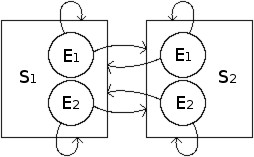
\includegraphics[width=4cm]{./evtstatmac.jpg}
\end{figure}
\end{center}

\subsection{Definition of the behaviour of the EvtStatMac}

The probabilities defining the behaviour of the EvtStatMac are: $P(e|s)$ (the probability for event $e$ to occur when the EvtStatMac is in status $s$) and $P(s'|e,s)$ (the probability to reach status $s'$ when the EvtStatMac is in status $s$ and event $e$ occurs).\\

If the behaviour of the EvtStatMac is learnt from sample data $\{(\bm{s},\bm{e},\bm{s'})\}$ (set of transitions from status $\bm{s}$ to status $\bm{s'}$ through event $\bm{e}$), the values of probabilities above are given by:\\
\begin{equation}
\label{eqnProbEvt}
P_{N_s}(e|s)=
\left\lbrace
\begin{array}{l}
0.0\textrm{, if }N_s = 0\\
\frac{N_{s,e}}{N_s}\textrm{, if }N_s \neq 0\textrm{ and }N_s<N^*\\
\frac{P_{N_s-1}(e|s)+1.0}{N^*+1.0}\textrm{, if }N_s\ge N^*\\
\end{array}
\right.
\end{equation}
and
\begin{equation}
\label{eqnProbTrans}
P_{N_s}(s'|s,e)=
\left\lbrace
\begin{array}{l}
0.0\textrm{, if }N_{s,e} = 0\\
\frac{N_{s,e,s'}}{N_{s,e}}\textrm{, if }N_{s,e} \neq 0\textrm{ and }N_{s,e}<N^*\\
\frac{P_{N_{s,e}-1}(s'|s,e)+1.0}{N^*+1.0}\textrm{, if }N_{s,e}\ge N^*\\
\end{array}
\right.
\end{equation}
where $N_{s}$ is the number of samples where $\bm{s}=s$; $N_{s,e}$ is the number of samples where $\bm{s}=s$ and $\bm{e}=e$; and $N_{s,e,s'}$ is the number of samples where $\bm{s}=s$, $\bm{e}=e$ and $\bm{s'}=s'$; $N^*$ is a maximum number of samples (to avoid overflow problem).\\

If the behaviour of the EvtStatMac is not learnt from sample data, we suppose the probabilities above are set manually by the user.\\

The EvtStatMac is normalized to ensure that:\\
\begin{equation}
\forall{s\in S},\sum_{e\in E}P(e|s)=1.0
\end{equation}
and 
\begin{equation}
\forall{s\in S},\forall{e\in E},P(e|s)\neq0.0\Rightarrow\sum_{s'\in S}P(s'|s,e)=1.0
\end{equation}
where $S$ is the set of possible status, and $E$ is the set of possible events.\\

\subsection{Reminder about probabilities}

We remind that:\\
\begin{equation}
P(A|B)=\frac{P(B|A)P(A)}{P(B)}
\end{equation}\\
\begin{equation}
P(A)=\sum_B\left[P(B)P(A|B)\right]
\end{equation}\\
\begin{equation}
P(A,B)=P(A|B)P(B)
\end{equation}\\
\begin{equation}
P(A,B)=P(B,A)
\end{equation}\\
\begin{equation}
P(A,B,C)=P(A)P(B|A)P(C|A,B)
\end{equation}\\

And we will also use the following equality (proof given in Annex 1):\\
\begin{equation}
P(e,s'|s)=P(s'|s,e)P(e|s)
\end{equation}

\subsection{Probabilities formulas}

Then, from probabilities (\ref{eqnProbEvt}) and (\ref{eqnProbTrans}) we can calculate the other probabilities below.\\

Probability to ends to status $s'$ after $n\in\mathbb{N}^+$ events starting from status $s$:\\
\begin{equation}
P_n(s'|s)=Q_n(s,s')
\end{equation}
where
$$
\left\lbrace
\begin{array}{l}
Q_0(s,s')=
\left\lbrace
\begin{array}{l}
1.0,s=s'\\
0.0,s\neq s'\\
\end{array}
\right.\\
Q_i(s,s')=\sum_{s''\in S}\left[\sum_{e\in E}\left[P(e|s'')P(s'|s'',e)Q_{i-1}(s,s'')\right]\right]
\end{array}
\right.
$$\\

Probability to be in status $s$:\\
\begin{equation}
P(s)=\lim_{i\rightarrow\infty}Q_i(s),i\in\mathbb{N}^+
\end{equation}
where
$$
\left\lbrace
\begin{array}{l}
Q_0(s')=\frac{1.0}{N_s}\\
Q_i(s')=\sum_{s\in S}\left[Q_{i-1}(s)P_1(s'|s)\right]
\end{array}
\right.
$$\\

Probability that event $e$ occurs:\\
\begin{equation}
P(e)=\sum_{s\in S}\left[P(s)P(e|s)\right]
\end{equation}\\

Probability that a transition from status $s$ through event $e$ occurs:\\
\begin{equation}
P(s,e)=P(e|s)P(s)
\end{equation}\\

Probability that a transition from status $s$ to status $s'$ occurs:\\
\begin{equation}
P(s,s')=P_1(s'|s)P(s)
\end{equation}\\

Probability that a transition to status $s'$ through event $e$ occurs:\\
\begin{equation}
\begin{array}{ll}
P(e,s')&=\sum_{s\in S}\left[P(e,s'|s)P(s)\right]\\
&=\sum_{s\in S}\left[P(s'|s,e)P(e|s)P(s)\right]\\
\end{array}
\end{equation}\\

Probability that a transition from status $s$ through event $e$ to status $s'$ occurs:\\
\begin{equation}
P(s,e,s')=P(s)P(e|s)P(s'|s,e)
\end{equation}\\

Probability that a transition started from status $s$ knowing that event $e$ occured:\\
\begin{equation}
P(s|e)=
\left\lbrace
\begin{array}{l}
\frac{P(e|s)P(s)}{P(e)}\textrm{, if }P(e) \neq 0.0\\
0.0\textrm{, if }P(e) = 0.0
\end{array}
\right.
\end{equation}\\

Probability that a transition started from status $s$ knowing that it has ended to status $s'$:\\
\begin{equation}
P(s|s')=
\left\lbrace
\begin{array}{l}
\frac{P_1(s'|s)P(s)}{P(s')}\textrm{, if }P(s') \neq 0.0\\
0.0\textrm{, if }P(s') = 0.0
\end{array}
\right.
\end{equation}\\

Probability that a transition ends to status $s'$ knowing that event $e$ occured:\\
\begin{equation}
P(s'|e)=
\left\lbrace
\begin{array}{l}
\frac{P(e,s')}{P(e)}\textrm{, if }P(e) \neq 0.0\\
0.0\textrm{, if }P(e) = 0.0
\end{array}
\right.
\end{equation}\\

Probability that a transition through event $e$ occured knowing that it ended to status $s'$:\\
\begin{equation}
P(e|s')=
\left\lbrace
\begin{array}{l}
\frac{P(e,s')}{P(s')}\textrm{, if }P(s') \neq 0.0\\
0.0\textrm{, if }P(s') = 0.0
\end{array}
\right.
\end{equation}\\

Probability that a transition started from status $s$ knowing that $e$ occured and ended to status $s'$:\\
\begin{equation}
P(s|e,s')=
\left\lbrace
\begin{array}{l}
\frac{P(s,e,s')}{P(e,s')}\textrm{, if }P(e,s') \neq 0.0\\
0.0\textrm{, if }P(e,s') = 0.0
\end{array}
\right.
\end{equation}\\

Probability that a transition through event $e$ occured knowing that it started from status $s$ and ended to status $s'$:\\
\begin{equation}
P(e|s,s')=
\left\lbrace
\begin{array}{l}
\frac{P(s,e,s')}{P(s,s')}\textrm{, if }P(s,s') \neq 0.0\\
0.0\textrm{, if }P(s,s') = 0.0
\end{array}
\right.
\end{equation}\\

\section{Interface}

\begin{scriptsize}
\begin{ttfamily}
\begin{lstlisting}
// *************** EVTSTATMAC.H ***************

#ifndef EVTSTATMAC_H
#define EVTSTATMAC_H

// ================= Include =================

#include <stdlib.h>
#include <stdio.h>
#include <math.h>
#include <string.h>
#include <stdbool.h>
#include <limits.h>

// ================= Define ==================

// Maximum number of samples when learning, to avoid overflow
#define ESM_NBMAXSAMPLE INT_MAX
// Null value for events and status
#define ESM_NULL -1
#define ESM_EVTNULL ESM_NULL
#define ESM_STATNULL ESM_NULL
// Precision
#define ESM_EPSILON 0.00000001
// Event type
#define esmEvt int
// State type
#define esmStat int

// ================= Data structure ===================

typedef struct EvtStatMac {
  // Number of possible statuss
  int _nbStatus;
  // Number of possible events
  int _nbEvent;
  // Number of learnt transitions for each status 
  int *_nbTransit;
  // Number of learnt occurence of each event for each status
  int *_nbEvt;
  // Number of learnt occurence of each status from each (status,event)
  int *_nbEvtToStat;
  // Probability of occurence of each event from each status
  float *_probEvt;
  // Probability of reaching each event from each (status,event)
  float *_probEvtToStat;
  // Initial status of the ESM
  esmStat _initState;
  // Current status of the ESM
  esmStat _curState;
  // Last occured event (updated by ESMStep...())
  esmEvt _lastEvt;
} EvtStatMac;

// ================ Functions declaration ====================

// Get a randomly choosen integer between 0 and 'nb' - 1 with a 
// probability for integer i to be choosen equal to 'prob[i]', 'prob' 
// must be normalized
// Return ESM_NULL if arguments are invalid
int ESMGetRnd(float *prob, int nb);

// Create, reset and init the ESM with 'nbState' possible status 
// and 'nbEvent' possible events, return NULL if the ESM couldn't 
// be created 
EvtStatMac* ESMCreate(esmStat initState, esmStat nbState, 
  esmEvt nbEvent);

// Clone a ESM, return NULL if the ESM couldn't be cloned
EvtStatMac* ESMClone(EvtStatMac *this);

// Load a ESM from a stream, return NULL if the ESM couldn't be loaded
EvtStatMac* ESMLoad(FILE *stream);

// Save a ESM to a stream, return false if the ESM couldn't be saved,
// true else
// Format:
// <_nbStatus>\n
// <_nbEvent>\n
// <_initState>\n
// for each status:
//   <_nbTransit[status]>\n
// for each status:
//   for each event:
//     <_nbEvt[status,event]>\n
// for each statusI:
//   for each event:
//     for each statusJ:
//       <_nbEvtToStat[statusI,event,statusJ]>\n
// for each status:
//   for each event:
//       <_probEvt[status,event]>\n
// for each statusI:
//   for each event:
//     for each statusJ:
//       <_probEvtToStat[statusI,event,statusJ]>\n
// <_curState>\n
// <_lastEvt>\n
bool ESMSave(EvtStatMac *this, FILE *stream);

// Init the ESM and reset all the probabilities of events to 
// 1.0/_nbEvent and all the probabilities of status to 1.0/_nbStatus
void ESMReset(EvtStatMac *this);

// Init the ESM and reset all the probabilities to 0.0
void ESMResetNull(EvtStatMac *this);

// Reset the current status to the initial status
void ESMInit(EvtStatMac *this);

// Normalize the probabilities
void ESMNormalize(EvtStatMac *this);

// Free the memory used by the ESM
void ESMFree(EvtStatMac **this);

// Print the ESM on 'stream'. If 'statLbl' and/or 'evtLbl' are not 
// null they are used as labels for status and events respectively 
// instead of printing their index
void ESMPrint(EvtStatMac *this, FILE *stream, char **statLbl, 
  char **evtLbl);

// Memorize one occurence of status 'to' after event 'event' from
// status 'from', and update all probabilities respectively
// ESMResetNull must be called before starting to learn
void ESMLearn(EvtStatMac *this, esmStat from, esmEvt event, esmStat to);

// Get the current status
// Return ESM_STATNULL if argument is invalid
esmStat ESMGetStat(EvtStatMac *this);

// Set the probability for 'event' to occur from status 'from'
void ESMSetPEvtGivFrom(EvtStatMac *this, esmStat from, esmEvt event, 
  float prob);

// Set the probability to be in status 'to' after 'event' occured 
// from status 'from'
void ESMSetPToGivFromEvt(EvtStatMac *this, esmStat from, esmEvt event, 
  esmStat to, float prob);

// Update the current status to a randomly choosen status from the
// current status
void ESMStep(EvtStatMac *this);

// Update the current status to a randomly choosen status given that 
// 'event' has occured from the current status
void ESMStepByEvt(EvtStatMac *this, esmEvt event);

// Get a randomly choosen event from the current status 
// Return ESM_EVTNULL if arguments are invalid
esmEvt ESMGetNextEvt(EvtStatMac *this);

// Get the last occured event 
// Return ESM_EVTNULL if arguments are invalid
esmEvt ESMGetLastEvt(EvtStatMac *this);

// Get a randomly choosen next status from the current status
// Return ESM_STATNULL if arguments are invalid
esmStat ESMGetNextStat(EvtStatMac *this);

// Get a randomly choosen next status given that 'event' has occured 
// from the current status
// Return ESM_STATNULL if arguments are invalid
esmStat ESMGetNextStatByEvt(EvtStatMac *this, esmEvt event);

// Get the probability that 'event' occurs from status 'from'
// Return 0.0 if arguments are invalid
float ESMGetPEvtGivFrom(EvtStatMac *this, esmStat from, esmEvt event);

// Get the probability that status 'to' occurs knowing 'event'
// occured after status 'from'
// Return 0.0 if arguments are invalid
float ESMGetPToGivFromEvt(EvtStatMac *this, esmStat from, esmEvt event, 
  esmStat to);

// Probability to ends to status 'to' after 'nbEvt' events starting 
// from status 'from'
// Return 0.0 if arguments are invalid
float ESMGetPToGivFrom(EvtStatMac *this, esmStat from, 
  esmStat to, int nbEvt);

// Probability to be in status 'status'
// Return 0.0 if arguments are invalid
float ESMGetPStatus(EvtStatMac *this, esmStat status);

// Probability that event 'event' occurs
// Return 0.0 if arguments are invalid
float ESMGetPEvent(EvtStatMac *this, esmEvt event);

// Probability that a transition from status 'from' through event 
// 'event' occurs
// Return 0.0 if arguments are invalid
float ESMGetPFromEvt(EvtStatMac *this, esmStat from, esmEvt event);

// Probability that a transition from status 'from' to status 'to' occurs
// Return 0.0 if arguments are invalid
float ESMGetPFromTo(EvtStatMac *this, esmStat from, esmStat to);

// Probability that a transition to status 'to' through event 'event' 
// occurs
// Return 0.0 if arguments are invalid
float ESMGetPEvtTo(EvtStatMac *this, esmEvt event, esmStat to);

// Probability that a transition from status 'from' through event 
// 'event' to status 'to' occurs
// Return 0.0 if arguments are invalid
float ESMGetPFromEvtTo(EvtStatMac *this, esmStat from, esmEvt event,
  esmStat to);

// Probability that a transition started from status 'from' knowing 
// that event 'event' occured
// Return 0.0 if arguments are invalid or P(event) = 0.0
float ESMGetPFromGivEvt(EvtStatMac *this, esmStat from, esmEvt event);

// Probability that a transition started from status 'from' knowing 
// that it has ended to status 'to'
// Return 0.0 if arguments are invalid or P(to) = 0.0
float ESMGetPFromGivTo(EvtStatMac *this, esmStat from, esmStat to);

// Probability that a transition ends to status 'to' knowing that 
// event 'event' occured
// Return 0.0 if arguments are invalid or P(event) = 0.0
float ESMGetPToGivEvt(EvtStatMac *this, esmEvt event, esmStat to);

// Probability that a transition through event 'event' occured
// knowing that it ended to status 'to'
// Return 0.0 if arguments are invalid or P(to) = 0.0
float ESMGetPEvtGivTo(EvtStatMac *this, esmEvt event, esmStat to);

// Probability that a transition started from status 'from' knowing 
// that 'event' occured and ended to status 'to'
// Return 0.0 if arguments are invalid or P(event, to) = 0.0
float ESMGetPFromGivEvtTo(EvtStatMac *this, esmStat from, esmEvt event,
  esmStat to);

// Probability that a transition through event 'event' occured knowing 
// that it started from status 'from' and ended to status 'to'
// Return 0.0 if arguments are invalid or P(from, to) = 0.0
float ESMGetPEvtGivFromTo(EvtStatMac *this, esmStat from, esmEvt event, 
  esmStat to);

#endif
\end{lstlisting}
\end{ttfamily}
\end{scriptsize}

\section{Code}

\begin{scriptsize}
\begin{ttfamily}
\begin{lstlisting}
// *************** EVTSTATMAC.C ***************

// ================= Include =================

#include "evtstatmac.h"

// ================= Define ==================

#define rnd() (double)(rand())/(float)(RAND_MAX)
#define ITRANSIT(s) (s)
#define IEVT(esm, s, e) ((s)*esm->_nbEvent+(e))
#define IEVTTOSTAT(esm, f, e, t) (IEVT(esm, f, e)*esm->_nbStatus+(t))

// ================ Functions implementation ==================

// Get a randomly choosen integer between 0 and 'nb' - 1 with a 
// probability for integer i to be choosen equal to 'prob[i]', 'prob' 
// must be normalized
// Return ESM_NULL if arguments are invalid
int ESMGetRnd(float *prob, int nb) {
  // Check arguments
  if (prob == NULL || nb <= 0) 
    return ESM_NULL;
  // Get a random value between 0 and 1
  float r = rnd();
  // Get the index 'ret' for which 
  // sum(prob[0..ret] <= r < sum(prob[0..ret+1]
  int ret = 0;
  float sum = 0.0;
  while (ret < nb && 
    !(sum >= r || r < sum + prob[ret])) {
    sum += prob[ret];
    ++ret;
  }
  if (ret < nb)
    return ret;
  else 
    return nb - 1;
}

// Create, reset and init the ESM with 'nbState' possible status 
// and 'nbEvent' possible events, return NULL if the ESM couldn't 
// be created 
EvtStatMac* ESMCreate(esmStat initState, esmStat nbState, 
  esmEvt nbEvent) {
  // Check arguments
  if (initState < 0 || initState >= nbState ||
    nbState <= 0 || nbEvent <= 0) 
    return NULL;
  // Allocate memory
  EvtStatMac *this = (EvtStatMac*)malloc(sizeof(EvtStatMac));
  if (this == NULL) return NULL;
  // Initialize properties with arguments
  this->_initState = initState;
  this->_nbStatus = nbState;
  this->_nbEvent = nbEvent;
  this->_lastEvt = ESM_EVTNULL;
  // Allocate memory for number of transition and probabilities
  this->_nbTransit = (int*)malloc(sizeof(int) * nbState);
  this->_nbEvt = (int*)malloc(sizeof(int) * nbState * nbEvent);
  this->_nbEvtToStat = 
    (int*)malloc(sizeof(int) * nbState * nbEvent * nbState);
  this->_probEvt = (float*)malloc(sizeof(float) * nbState * nbEvent);
  this->_probEvtToStat = 
    (float*)malloc(sizeof(float) * nbState * nbEvent * nbState);
  if (this->_nbTransit == NULL || this->_nbEvt == NULL || 
    this->_nbEvtToStat == NULL || this->_probEvt == NULL || 
    this->_probEvtToStat == NULL)
    ESMFree(&this);
  // Reset the number of transitions and probabilities
  ESMReset(this);
  // Return the new EvtStatMac
  return this;
}

// Clone a ESM, return NULL if the ESM couldn't be cloned
EvtStatMac* ESMClone(EvtStatMac *this) {
  // Check arguments
  if (this == NULL) 
    return NULL;
  // Create a EvtStatMac with the same arguments as the one in argument
  EvtStatMac *c = 
    ESMCreate(this->_initState, this->_nbStatus, this->_nbEvent);
  if (c != NULL) {
    // Copy the number of transition and probabilities
    memcpy(c->_nbTransit, this->_nbTransit, sizeof(int) * this->_nbStatus);
    memcpy(c->_nbEvt, this->_nbEvt, 
      sizeof(int) * this->_nbStatus * this->_nbEvent);
    memcpy(c->_nbEvtToStat, this->_nbEvtToStat, 
      sizeof(int) * this->_nbStatus * this->_nbEvent * this->_nbStatus);
    memcpy(c->_probEvt, this->_probEvt, 
      sizeof(int) * this->_nbStatus * this->_nbEvent);
    memcpy(c->_probEvtToStat, this->_probEvtToStat, 
      sizeof(int) * this->_nbStatus * this->_nbEvent * this->_nbStatus);
  }
  // Return the cloned EvtStatMac
  return c;
}

// Load a ESM from a stream, return NULL if the ESM couldn't be loaded
EvtStatMac* ESMLoad(FILE *stream) {
  // Check arguments
  if (stream == NULL) 
    return NULL;

  // Read the number of statuss and events and initial status
  int nbState;
  int nbEvent;
  int initState;
  if (fscanf(stream, "%d", &nbState) == EOF)
    return NULL;
  if (fscanf(stream, "%d", &nbEvent) == EOF)
    return NULL;
  if (fscanf(stream, "%d", &initState) == EOF)
    return NULL;
  // Create a EvtStatMac
  EvtStatMac *this = ESMCreate(initState, nbState, nbEvent);
  if (this == NULL)
    return NULL;
  // Read the values of all the properties of the EVM structure
  for (int iStat = 0; iStat < this->_nbStatus; ++iStat)
    if (fscanf(stream, "%d", 
      &(this->_nbTransit[ITRANSIT(iStat)])) == EOF) {
      ESMFree(&this);
      return NULL;
    }
  for (int iStat = 0; iStat < this->_nbStatus; ++iStat)
    for (int iEvt = 0; iEvt < this->_nbEvent; ++iEvt)
      if (fscanf(stream, "%d", 
        &(this->_nbEvt[IEVT(this, iStat, iEvt)])) == EOF) {
        ESMFree(&this);
        return NULL;
      }
  for (int iStat = 0; iStat < this->_nbStatus; ++iStat)
    for (int iEvt = 0; iEvt < this->_nbEvent; ++iEvt)
      for (int jStat = 0; jStat < this->_nbStatus; ++jStat)
        if (fscanf(stream, "%d", 
          &(this->_nbEvtToStat[
          IEVTTOSTAT(this, iStat, iEvt, jStat)])) == EOF) {
          ESMFree(&this);
          return NULL;
        }
  for (int iStat = 0; iStat < this->_nbStatus; ++iStat)
    for (int iEvt = 0; iEvt < this->_nbEvent; ++iEvt)
      if (fscanf(stream, "%f", 
        &(this->_probEvt[IEVT(this, iStat, iEvt)])) == EOF) {
        ESMFree(&this);
        return NULL;
      }
  for (int iStat = 0; iStat < this->_nbStatus; ++iStat)
    for (int iEvt = 0; iEvt < this->_nbEvent; ++iEvt)
      for (int jStat = 0; jStat < this->_nbStatus; ++jStat)
        if (fscanf(stream, "%f", 
          &(this->_probEvtToStat[
          IEVTTOSTAT(this, iStat, iEvt, jStat)])) == EOF) {
          ESMFree(&this);
          return NULL;
        }
  if (fscanf(stream, "%d", &(this->_curState)) == EOF) {
    ESMFree(&this);
    return NULL;
  }
  if (fscanf(stream, "%d", &(this->_lastEvt)) == EOF) {
    ESMFree(&this);
    return NULL;
  }
  // Return the cloned EvtStatMac
  return this;
}

// Save a ESM to a stream, return false if the ESM couldn't be saved,
// true else
bool ESMSave(EvtStatMac *this, FILE *stream) {
  // Check arguments
  if (this == NULL || stream == NULL) 
    return false;
  // Save the values of all the properties of the EVM structure
  if (fprintf(stream, "%d\n", this->_nbStatus) < 0)
    return false;
  if (fprintf(stream, "%d\n", this->_nbEvent) < 0)
    return false;
  if (fprintf(stream, "%d\n", this->_initState) < 0)
    return false;
  for (int iStat = 0; iStat < this->_nbStatus; ++iStat)
    if (fprintf(stream, "%d\n", this->_nbTransit[ITRANSIT(iStat)]) < 0)
      return false;
  for (int iStat = 0; iStat < this->_nbStatus; ++iStat)
    for (int iEvt = 0; iEvt < this->_nbEvent; ++iEvt)
      if (fprintf(stream, "%d\n", 
        this->_nbEvt[IEVT(this, iStat, iEvt)]) < 0)
        return false;
  for (int iStat = 0; iStat < this->_nbStatus; ++iStat)
    for (int iEvt = 0; iEvt < this->_nbEvent; ++iEvt)
      for (int jStat = 0; jStat < this->_nbStatus; ++jStat)
        if (fprintf(stream, "%d\n", 
          this->_nbEvtToStat[IEVTTOSTAT(this, iStat, iEvt, jStat)]) < 0)
          return false;
  for (int iStat = 0; iStat < this->_nbStatus; ++iStat)
    for (int iEvt = 0; iEvt < this->_nbEvent; ++iEvt)
      if (fprintf(stream, "%f\n", 
        this->_probEvt[IEVT(this, iStat, iEvt)]) < 0)
        return false;
  for (int iStat = 0; iStat < this->_nbStatus; ++iStat)
    for (int iEvt = 0; iEvt < this->_nbEvent; ++iEvt)
      for (int jStat = 0; jStat < this->_nbStatus; ++jStat)
        if (fprintf(stream, "%f\n", 
          this->_probEvtToStat[IEVTTOSTAT(
          this, iStat, iEvt, jStat)]) < 0)
          return false;
  if (fprintf(stream, "%d\n", this->_curState) < 0)
    return false;
  if (fprintf(stream, "%d\n", this->_lastEvt) < 0)
    return false;
  // Return true to signify success
  return true;
}

// Init the ESM and reset all the probabilities of events to 
// 1.0/_nbEvent and all the probabilities of status to 1.0/_nbStatus
void ESMReset(EvtStatMac *this) {
  // Check arguments
  if (this == NULL) 
    return;
  // Init the status
  ESMInit(this);
  // For each possible status 'from'
  for (esmStat iStat = this->_nbStatus; iStat--;) {
    // Reset the number of transition from status 'from'
    this->_nbTransit[ITRANSIT(iStat)] = 0;
    // For each possible event
    for (esmEvt iEvt = this->_nbEvent; iEvt--;) {
      // Reset the number of transition ('from', 'event')
      this->_nbEvt[IEVT(this, iStat, iEvt)] = 0;
      // Reset the probability of transition ('from', 'event') to 
      // 1/_nbEvent
      this->_probEvt[IEVT(this, iStat, iEvt)] = 
        1.0 / (float)(this->_nbEvent);
      // For each possible status 'to'
      for (esmStat jStat = this->_nbStatus; jStat--;) {
        // Reset the number of transition ('from', 'event', 'to')
        this->_nbEvtToStat[IEVTTOSTAT(this, iStat, iEvt, jStat)] = 0;
        // Reset the probability of transition ('from', 'event', 'to') 
        // to 1/_nbStatus
        this->_probEvtToStat[IEVTTOSTAT(this, iStat, iEvt, jStat)] = 
          1.0 / (float)(this->_nbStatus);
      }
    }
  }
}

// Init the ESM and reset all the probabilities to 0.0
void ESMResetNull(EvtStatMac *this) {
  // Check arguments
  if (this == NULL) 
    return;
  // Init the status
  ESMInit(this);
  // For each possible status 'from'
  for (esmStat iStat = this->_nbStatus; iStat--;) {
    // Reset the number of transition from status 'from'
    this->_nbTransit[ITRANSIT(iStat)] = 0;
    // For each possible event
    for (esmEvt iEvt = this->_nbEvent; iEvt--;) {
      // Reset the number of event from status 'from'
      this->_nbEvt[IEVT(this, iStat, iEvt)] = 0;
      // Reset the probqbility of event 'event' from status 'from'
      this->_probEvt[IEVT(this, iStat, iEvt)] = 0.0;
      // For each possible status 'to'
      for (esmStat jStat = this->_nbStatus; jStat--;) {
        // Reset the number of transition ('from', 'event', 'to')
        this->_nbEvtToStat[IEVTTOSTAT(this, iStat, iEvt, jStat)] = 0;
        // Reset the probability of transition ('from', 'event', 'to')
        this->_probEvtToStat[IEVTTOSTAT(this, iStat, iEvt, jStat)] = 0.0;
      }
    }
  }
}

// Reset the current status to the initial status
void ESMInit(EvtStatMac *this) {
  // Check arguments
  if (this == NULL) 
    return;
  // Set the current status to the initial status
  this->_curState = this->_initState;  
}

// Normalize the probabilities
void ESMNormalize(EvtStatMac *this) {
  // Check arguments
  if (this == NULL) 
    return;
  // For each possible status 'from'
  for (esmStat iStat = this->_nbStatus; iStat--;) {
    // variable to memorize the sum of probabilities
    float sum = 0.0;
    // For each possible event
    for (esmEvt iEvt = this->_nbEvent; iEvt--;) {
      // Reset the sum of probabilities
      sum = 0.0;
      // For each possible status 'to'
      for (esmStat jStat = this->_nbStatus; jStat--;)
        // Sum the probability of ('from', 'event', 'to')
        sum += 
          this->_probEvtToStat[IEVTTOSTAT(this, iStat, iEvt, jStat)];
      // If the sum is not null 
      if (sum > ESM_EPSILON)
        // For each status 'to'
        for (esmStat jStat = this->_nbStatus; jStat--;)
          // Normalize the probability of ('from', 'event', 'to') by 
          // dividing by the sum of probabilities
          this->_probEvtToStat[IEVTTOSTAT(this, iStat, iEvt, jStat)] /=
            sum;
      // Else, the sum of probabilities is null
      else
        // It means this event never occurs,
        // set its probability to 0
        this->_probEvt[IEVT(this, iStat, iEvt)] = 0.0;
    }
    // Reset the sum of probability
    sum = 0.0;
    // For each possible event
    for (esmEvt iEvt = this->_nbEvent; iEvt--;)
      // Sum the probability of this event
      sum += this->_probEvt[IEVT(this, iStat, iEvt)];
    // If the sum is not null
    if (sum > ESM_EPSILON)
      // For each possible event
      for (esmEvt iEvt = this->_nbEvent; iEvt--;)
        // Normalize the probability of ('from', 'event') by dividing 
        // by the sum of probabilities
        this->_probEvt[IEVT(this, iStat, iEvt)] /= sum;
  }
}

// Free the memory used by the ESM
void ESMFree(EvtStatMac **this) {
  // Check arguments
  if (this == NULL || *this == NULL) 
    return;
  // Free the memory
  if ((*this)->_nbTransit != NULL) {
    free((*this)->_nbTransit);
    (*this)->_nbTransit = NULL;
  }
  if ((*this)->_nbEvt != NULL) {
    free((*this)->_nbEvt);
    (*this)->_nbEvt = NULL;
  }
  if ((*this)->_nbEvtToStat != NULL) {
    free((*this)->_nbEvtToStat);
    (*this)->_nbEvtToStat = NULL;
  }
  if ((*this)->_probEvt != NULL) {
    free((*this)->_probEvt);
    (*this)->_probEvt = NULL;
  }
  if ((*this)->_probEvtToStat != NULL) {
    free((*this)->_probEvtToStat);
    (*this)->_probEvtToStat = NULL;
  }
  free(*this);
  *this = NULL;
}

// Print the ESM on 'stream'. If 'statLbl' and/or 'evtLbl' are not 
// null they are used as labels for status and events respectively 
// instead of printing their index
void ESMPrint(EvtStatMac *this, FILE *stream, char **statLbl, 
  char **evtLbl) {
  // Check arguments
  if (this == NULL || stream == NULL) 
    return;
  // If there is no labels for the status
  if (statLbl == NULL)
    // Print the index of the current status
    fprintf(stream, "current status: %d\n", this->_curState);
  // Else, if the current status has a valid index
  else if (this->_curState >= 0 && this->_curState < this->_nbStatus)
    // Print the label of the current status
    fprintf(stream, "current status: '%s'\n", statLbl[this->_curState]);
  // Else, the current status is not a valid index
  else 
    // Print the current status
    fprintf(stream, "current status: (null, %d)\n", this->_curState);
  // For each possible status
  for (int from = 0; from < this->_nbStatus; ++from) {
    // If there is no labels for the status
    if (statLbl == NULL)
      // Print the index of the status 'from'
      fprintf(stream, "from status #%d:\n", from);
    // Else, if the status 'from' has a valid index
    else if (from >= 0 && from < this->_nbStatus)
      // Print the label of the status 'from'
      fprintf(stream, "from status '%s'\n", statLbl[from]);
    // Else, the status 'from' is not a valid index
    else 
      // Print the status 'from'
      fprintf(stream, "from status (null, %d)\n", from);
    // Flag to memorize if there is occurences from the status 'from'
    bool flagOccurence = false;
    // For each possible event
    for (int event = 0; event < this->_nbEvent; ++event) {
      // Get the probability of this event from the status 'from'
      float p = ESMGetPEvtGivFrom(this, from, event);
      // If the probability is not null
      if (p > ESM_EPSILON) {
        // Memorize that there is occurence from the status 'from'
        flagOccurence = true;
        // If there is no label for the events
        if (evtLbl == NULL)
          // Print the index of the event
          fprintf(stream, "  by event #%d (%f):\n", event, p);
        // Else, if the index of the event is valid
        else if (event >= 0 && event < this->_nbEvent)
          // Print the label of the event
          fprintf(stream, "  by event '%s' (%f):\n", evtLbl[event], p);
        // Else, the index of the event is not valid
        else
          // Print the event
          fprintf(stream, "  by event (null, %d) (%f):\n", event, p);
        // For each status 'to'
        for (int to = 0; to < this->_nbStatus; ++to) {
          // Get the probability of ('from', 'event', 'to')
          float q = ESMGetPToGivFromEvt(this, from, event, to);
          // If the probability is not null
          if (q > ESM_EPSILON) {
            // If there is no label for the status
            if (statLbl == NULL)
              // Print the index of the status 'to'
              fprintf(stream, "    -> status #%d (%f)\n", to, q);
            // Else, if the index for the status 'to' is valid
            else if (to >= 0 && to < this->_nbStatus)
              // Print the label of the status 'to'
              fprintf(stream, "    -> status '%s' (%f)\n", 
                statLbl[to], q);
            // Else, the index of the status is not valid
            else
              // Print the the status 'to'
              fprintf(stream, "    -> status (null, %d) (%f)\n", 
                to, q);
          }
        }
      }
    }
    // If there was no transit from the status 'from'
    if (flagOccurence == false)
      // Print an appropriate message
      fprintf(stream, "  no transit from this status\n");
  }
}

// Memorize one occurence of status 'to' after event 'event' from
// status 'from', and update all probabilities respectively
// ESMResetNull must be called before starting to learn
void ESMLearn(EvtStatMac *this, esmStat from, esmEvt event, 
  esmStat to) {
  // Check arguments
  if (this == NULL || event < 0 || event >= this->_nbEvent ||
    from < 0 || from >= this->_nbStatus ||
    to < 0 || to >= this->_nbStatus)
    return;
  // If we haven't reached the maximum number of samples
  if (this->_nbTransit[ITRANSIT(from)] < ESM_NBMAXSAMPLE) {
    // Update the number of transition for the status 'from'
    ++(this->_nbTransit[ITRANSIT(from)]);
    // Update the number of events for the status 'from'
    ++(this->_nbEvt[IEVT(this, from, event)]);
    // Update the number of transition for ('from', 'event');
    ++(this->_nbEvtToStat[IEVTTOSTAT(this, from, event, to)]);
    // Calculate the new probability for ('from', 'event')
    float p = (float)(this->_nbEvt[IEVT(this, from, event)]) / 
      (float)(this->_nbTransit[ITRANSIT(from)]);
    // Set the probability
    ESMSetPEvtGivFrom(this, from, event, p);
    // Calculate the new probability for ('from', 'event', 'to')
    float q = 
      (float)(this->_nbEvtToStat[IEVTTOSTAT(this, from, event, to)]) / 
      (float)(this->_nbEvt[IEVT(this, from, event)]);
    // Set the probability
    ESMSetPToGivFromEvt(this, from, event, to, q);
    // Keep the probabilities normalized
    ESMNormalize(this);
  // Else, if we have reached the maximum number of samples
  } else {
    // Calculate the new probability for ('from', 'event')
    float p = (ESMGetPEvtGivFrom(this, from, event) * 
      (float)(this->_nbTransit[ITRANSIT(from)]) + 1.0) / 
      ((float)(this->_nbTransit[ITRANSIT(from)]) + 1.0);
    // Set the probability
    ESMSetPEvtGivFrom(this, from, event, p);
    // Calculate the new probability for ('from', 'event', 'to')
    float q = (ESMGetPToGivFromEvt(this, from, event, to) * 
      (float)(this->_nbEvt[IEVT(this, from, event)]) + 1.0) / 
      ((float)(this->_nbEvt[IEVT(this, from, event)]) + 1.0);
    // Set the probability
    ESMSetPToGivFromEvt(this, from, event, to, q);
    // Keep the probabilities normalized
    ESMNormalize(this);
    // Correct the number of events for the status 'from'
    // to keep _nbEvt coherent with probability for ('from', 'event')
    this->_nbEvt[IEVT(this, from, event)] = 
      (int)round(p * (float)(this->_nbTransit[ITRANSIT(from)]));
    // Correct the number of events for the status 'from'
    // to keep _nbEvtToStat coherent with _nbEvt and 
    // probability for ('from', 'event', 'to')
    this->_nbEvtToStat[IEVTTOSTAT(this, from, event, to)] = 
      (int)round(q * (float)(this->_nbEvt[IEVT(this, from, event)]));
  }
}

// Get the current status
// Return ESM_STATNULL if argument is invalid
esmStat ESMGetStat(EvtStatMac *this) {
  // Check arguments
  if (this == NULL) 
    return ESM_STATNULL;
  // Return the current status
  return this->_curState;  
}

// Set the probability for 'event' to occur from status 'from'
void ESMSetPEvtGivFrom(EvtStatMac *this, esmStat from, esmEvt event, 
  float prob) {
  // Check arguments
  if (this == NULL || event < 0 || event >= this->_nbEvent ||
    from < 0 || from >= this->_nbStatus || prob < 0.0) 
    return;
  // Set the probability
  this->_probEvt[IEVT(this, from, event)] = prob;
}

// Set the probability to be in status 'to' after 'event' occured 
// from status 'from'
void ESMSetPToGivFromEvt(EvtStatMac *this, esmStat from, esmEvt event, 
  esmStat to, float prob) {
  // Check arguments
  if (this == NULL || event < 0 || event >= this->_nbEvent ||
    from < 0 || from >= this->_nbStatus ||
    to < 0 || to >= this->_nbStatus || prob < 0.0) 
    return;
  // Set the probability
  this->_probEvtToStat[IEVTTOSTAT(this, from, event, to)] = prob;
}

// Update the current status to a randomly choosen status from the
// current status
void ESMStep(EvtStatMac *this) {
  // Check arguments
  if (this == NULL) 
    return;
  // Set the current status to a randomly choosen status from the 
  // current status via a randomly choosen event according to 
  // memorized probabilities
  this->_lastEvt = ESMGetNextEvt(this);
  this->_curState = ESMGetNextStatByEvt(this, this->_lastEvt);
}

// Update the current status to a randomly choosen status given that 
// 'event' has occured from the current status
void ESMStepByEvt(EvtStatMac *this, int event) {
  // Check arguments
  if (this == NULL || event < 0 || event >= this->_nbEvent) 
    return;
  // Set the current status to a randomly choosen status from the 
  // current status via the requested event according to 
  // memorized probabilities
  this->_curState = ESMGetNextStatByEvt(this, event);
  this->_lastEvt = event;
}

// Get a randomly choosen event from the current status 
// Return ESM_EVTNULL if arguments are invalid
esmEvt ESMGetNextEvt(EvtStatMac *this) {
  // Check arguments
  if (this == NULL || this->_curState < 0 || 
    this->_curState >= this->_nbStatus) 
    return ESM_EVTNULL;
  // Return a randomly choosen event according to memorized 
  // probabilities of events from the current status
  return ESMGetRnd(this->_probEvt + IEVT(this, this->_curState, 0), 
    this->_nbEvent);
}

// Get the last occured event 
// Return ESM_EVTNULL if arguments are invalid
esmEvt ESMGetLastEvt(EvtStatMac *this) {
  // Check arguments
  if (this == NULL) 
    return ESM_EVTNULL;
  // Return the last event
  return this->_lastEvt;
}

// Get a randomly choosen next status from the current status
// Return ESM_STATNULL if arguments are invalid
esmStat ESMGetNextStat(EvtStatMac *this) {
  // Check arguments
  if (this == NULL) return ESM_STATNULL;
  // Return a randomly choosen status from the current status via 
  // a randomly choosen event according to memorized probabilities
  return ESMGetNextStatByEvt(this, ESMGetNextEvt(this));
}

// Get a randomly choosen next status given that 'event' has occured 
// from the current status
// Return ESM_STATNULL if arguments are invalid
esmStat ESMGetNextStatByEvt(EvtStatMac *this, esmEvt event) {
  // Check arguments
  if (this == NULL || event < 0 || event >= this->_nbEvent ||
    this->_curState < 0 || this->_curState >= this->_nbStatus) 
    return ESM_STATNULL;
  // Return a randomly choosen status according to memorized 
  // probabilities of status from the current status via the requested
  // event
  return ESMGetRnd( 
    this->_probEvtToStat + 
    IEVTTOSTAT(this, this->_curState, event, 0), 
    this->_nbStatus);
}

// Get the probability that 'event' will occur from status 'from'
// Return 0.0 if arguments are invalid
float ESMGetPEvtGivFrom(EvtStatMac *this, esmStat from, 
  esmEvt event) {
  // Check arguments
  if (this == NULL || event < 0 || event >= this->_nbEvent ||
    from < 0 || from >= this->_nbStatus) 
    return 0.0;
  // Return the memorized probability
  return this->_probEvt[IEVT(this, from, event)];
}

// Get the probability that status 'to' occured knowing 'event'
// occured after status 'from'
// Return 0.0 if arguments are invalid
float ESMGetPToGivFromEvt(EvtStatMac *this, esmStat from, esmEvt event, 
  esmStat to) {
  // Check arguments
  if (this == NULL || event < 0 || event >= this->_nbEvent ||
    from < 0 || from >= this->_nbStatus ||
    to < 0 || to >= this->_nbStatus) 
    return 0.0;
  // Return the memorized probability
  return this->_probEvtToStat[IEVTTOSTAT(this, from, event, to)];  
}

// Recursive function for ESMGetProbStatByStat
float ESMGetPToGivFromRec(EvtStatMac *this, esmStat from, esmStat to, 
  int nbEvt) {
  // Variable to memorize the probability
  double prob = 0.0;
  // If we have reach the requested number of event and we are at the
  // requested 'from' status
  if (from == to && nbEvt == 0) {
    // Return a probability of 1.0, which will sum up the probability 
    // down to this point
    prob = 1.0;
  // Else, if we haven't reach yet the requested number of event
  // keep checking the possible transition leading to the status 'to'
  } else if (nbEvt > 0) {
    // For each possible status
    for (esmStat iStat = this->_nbStatus; iStat--;) {
      // For each possible event
      for (esmEvt iEvt = this->_nbEvent; iEvt--;) {
        // Get the probability for the transition (iStat, iEvt, to)
        float p = this->_probEvt[IEVT(this, iStat, iEvt)] * 
          this->_probEvtToStat[IEVTTOSTAT(this, iStat, iEvt, to)];
        // If the probability for this transition is not null
        if (p > ESM_EPSILON) {
          // Go back one more event seaching for transitions going 
          // to iStat, multiply by the probability of these transition
          // and add to the total probability
          p *= ESMGetPToGivFromRec(this, from, iStat, nbEvt - 1);
          prob += p;
        }
      }
    }
  }
  // Return the result probability
  return prob;
}

// Probability to ends to status 'to' after 'nbEvt' events starting 
// from status 'from'
// Return 0.0 if arguments are invalid
float ESMGetPToGivFrom(EvtStatMac *this, esmStat from, esmStat to, 
  int nbEvt) {
  // Check arguments
  if (this == NULL || from < 0 || from >= this->_nbStatus ||
    to < 0 || to >= this->_nbStatus) 
    return 0.0;
  // Start the recursion
  double p = ESMGetPToGivFromRec(this, from, to, nbEvt);
  // Return the probability
  return p;
}

// Probability to be in status 'status'
// Return 0.0 if arguments are invalid
float ESMGetPStatus(EvtStatMac *this, esmStat status) {
  // Check arguments
  if (this == NULL || status < 0 || status >= this->_nbStatus) 
    return 0.0;
  // Variable to memorize the delta between probability for ending
  // condition of the loop
  float dprob = 0.0;
  // Allocate memory for the calculated probabilities of each status
  float *prior = (float*)malloc(sizeof(float) * this->_nbStatus);
  if (prior == NULL) return 0.0;
  // Initialize the probability of each status to 1/_nbStatus
  // (consider all status as equally probable by defaut) 
  for (int iStat = this->_nbStatus; iStat--;)
    prior[iStat] = 1.0 / (float)(this->_nbStatus);
  // Allocate memory for the new calculated probability of each status
  float *nprior = (float*)malloc(sizeof(float) * this->_nbStatus);
  if (nprior == NULL) {
    free(prior);
    return 0.0;
  }
  // Security to avoid infinite loop
  int nbMaxIter = 10000;
  // Loop to calculate the limit
  do {
    // For each possible status 'to'
    for (int iStat = this->_nbStatus; iStat--;) {
      // Set the new probability of this status to 0.0
      nprior[iStat] = 0.0;
      // For each possible status 'from'
      for (int jStat = this->_nbStatus; jStat--;)
        // Sum the probability of transition from 'from' to 'to'
        // multiplied by the probability of 'from'
        nprior[iStat] += prior[jStat] * 
          ESMGetPToGivFrom(this, jStat, iStat, 1);
    }
    // For each possible status
    for (int iStat = this->_nbStatus; iStat--;) {
      // If it's the requested status
      if (iStat == status)
        // Memorize the delta between current probability and new
        // probability
        dprob = fabs(nprior[iStat] - prior[iStat]);
      // Update the probability of this status with the newly calculated
      // probability
      prior[iStat] = nprior[iStat];
    }
    --nbMaxIter;
  // Loop until the probability of the requested status is not stable
  } while (dprob > ESM_EPSILON && nbMaxIter > 0);
  // Memorize the probability of the requested status
  float prob = prior[status];
  // Free memory
  free(prior);
  free(nprior);
  // Return the result probability
  return prob;
}

// Probability that event 'event' occurs
// Return 0.0 if arguments are invalid
float ESMGetPEvent(EvtStatMac *this, esmEvt event) {
  // Check arguments
  if (this == NULL || event < 0 || event >= this->_nbEvent) 
    return 0.0;
  // Variable to memorize the result probability
  float prob = 0.0;
  // For each possible status
  for (int iStat = this->_nbStatus; iStat--;)
    // Sum the probability of the event frm this status multiplied
    // by the probability of this status
    prob += ESMGetPStatus(this, iStat) * 
      ESMGetPEvtGivFrom(this, iStat, event);
  // Return the result probability
  return prob;
}

// Probability that a transition from status 'from' through event 
// 'event' occurs
// Return 0.0 if arguments are invalid
float ESMGetPFromEvt(EvtStatMac *this, esmStat from, esmEvt event) {
  // Check arguments
  if (this == NULL || from < 0 || from >= this->_nbStatus ||
    event < 0 || event >= this->_nbEvent) 
    return 0.0;
  return ESMGetPEvtGivFrom(this, from, event) * 
    ESMGetPStatus(this, from);
}

// Probability that a transition from status 'from' to status 'to' occurs
// Return 0.0 if arguments are invalid
float ESMGetPFromTo(EvtStatMac *this, esmStat from, esmStat to) {
  // Check arguments
  if (this == NULL || from < 0 || from >= this->_nbStatus ||
    to < 0 || to >= this->_nbStatus) 
    return 0.0;
  return ESMGetPToGivFrom(this,from, to, 1) * 
    ESMGetPStatus(this, from);
}

// Probability that a transition to status 'to' through event 'event' 
// occurs
// Return 0.0 if arguments are invalid
float ESMGetPEvtTo(EvtStatMac *this, esmEvt event, esmStat to) {
  // Check arguments
  if (this == NULL || event < 0 || event >= this->_nbEvent ||
    to < 0 || to >= this->_nbStatus) 
    return 0.0;
  float p = 0.0;
  for (int iStat = this->_nbStatus; iStat--;)
    p += ESMGetPToGivFromEvt(this, iStat, event, to) * 
      ESMGetPEvtGivFrom(this, iStat, event) * 
      ESMGetPStatus(this, iStat);
  return p;
}

// Probability that a transition from status 'from' through event 
// 'event' to status 'to' occurs
// Return 0.0 if arguments are invalid
float ESMGetPFromEvtTo(EvtStatMac *this, esmStat from, esmEvt event,
  esmStat to) {
  // Check arguments
  if (this == NULL || from < 0 || from >= this->_nbStatus ||
    event < 0 || event >= this->_nbEvent ||
    to < 0 || to >= this->_nbStatus) 
    return 0.0;
  return ESMGetPStatus(this, from) * 
    ESMGetPEvtGivFrom(this, from, event) *
    ESMGetPToGivFromEvt(this, from, event, to);
}

// Probability that a transition started from status 'from' knowing 
// that event 'event' occured
// Return 0.0 if arguments are invalid or P(event) = 0.0 
float ESMGetPFromGivEvt(EvtStatMac *this, esmStat from, esmEvt event) {
  // Check arguments
  if (this == NULL || from < 0 || from >= this->_nbStatus ||
    event < 0 || event >= this->_nbEvent) 
    return 0.0;
  float d = ESMGetPEvent(this, event);
  if (d > ESM_EPSILON)
    return ESMGetPEvtGivFrom(this, from, event) * 
      ESMGetPStatus(this, from) / d;
  else
    return 0.0;
}

// Probability that a transition started from status 'from' knowing 
// that it has ended to status 'to'
// Return 0.0 if arguments are invalid or P(to) = 0.0
float ESMGetPFromGivTo(EvtStatMac *this, esmStat from, esmStat to) {
  // Check arguments
  if (this == NULL || from < 0 || from >= this->_nbStatus ||
    to < 0 || to >= this->_nbStatus) 
    return 0.0;
  float d = ESMGetPStatus(this, to);
  if (d > ESM_EPSILON)
    return ESMGetPToGivFrom(this, from, to, 1) * 
      ESMGetPStatus(this, from) / d;
  else
    return 0.0;
}

// Probability that a transition ends to status 'to' knowing that 
// event 'event' occured
// Return 0.0 if arguments are invalid or P(event) = 0.0
float ESMGetPToGivEvt(EvtStatMac *this, esmEvt event, esmStat to) {
  // Check arguments
  if (this == NULL || event < 0 || event >= this->_nbEvent ||
    to < 0 || to >= this->_nbStatus) 
    return 0.0;
  float d = ESMGetPEvent(this, event);
  if (d > ESM_EPSILON)
    return ESMGetPEvtTo(this, event, to) / d;
  else
    return 0.0;
}

// Probability that a transition through event 'event' occured knowing that it ended to status 'to'
// Return 0.0 if arguments are invalid or P(to) = 0.0
float ESMGetPEvtGivTo(EvtStatMac *this, esmEvt event, esmStat to) {
  // Check arguments
  if (this == NULL || event < 0 || event >= this->_nbEvent ||
    to < 0 || to >= this->_nbStatus) 
    return 0.0;
  float d = ESMGetPStatus(this, to);
  if (d > ESM_EPSILON)
    return ESMGetPEvtTo(this, event, to) / d;
  else
    return 0.0;
}

// Probability that a transition started from status 'from' knowing 
// that 'event' occured and ended to status 'to'
// Return 0.0 if arguments are invalid or P(event, to) = 0.0
float ESMGetPFromGivEvtTo(EvtStatMac *this, esmStat from, esmEvt event,
  esmStat to) {
  // Check arguments
  if (this == NULL || from < 0 || from >= this->_nbStatus ||
    event < 0 || event >= this->_nbEvent ||
    to < 0 || to >= this->_nbStatus) 
    return 0.0;
  float d = ESMGetPEvtTo(this, event, to);
  if (d > ESM_EPSILON)
    return ESMGetPFromEvtTo(this, from, event, to) / d;
  else
    return 0.0;
}

// Probability that a transition through event 'event' occured knowing 
// that it started from status 'from' and ended to status 'to'
// Return 0.0 if arguments are invalid or P(from, to) = 0.0
float ESMGetPEvtGivFromTo(EvtStatMac *this, esmStat from, 
  esmEvt event, esmStat to) {
  // Check arguments
  if (this == NULL || event < 0 || event >= this->_nbEvent ||
    from < 0 || from >= this->_nbStatus ||
    to < 0 || to >= this->_nbStatus) 
    return 0.0;
  float d = ESMGetPFromTo(this, from, to);
  if (d > ESM_EPSILON)
    return ESMGetPFromEvtTo(this, from, event, to) / d;
  else
    return 0.0;
}
\end{lstlisting}
\end{ttfamily}
\end{scriptsize}

\section{Usage}

\subsection{Code}

\begin{scriptsize}
\begin{ttfamily}
\begin{lstlisting}
#include <stdlib.h>
#include <stdio.h>
#include <math.h>
#include <time.h>
#include "evtstatmac.h"

#define rnd() (double)(rand())/(float)(RAND_MAX)

#define NBMAXSTAT 5
#define NBMAXEVT 5
#define NBSAMPLE 1000000
#define EPSILON 0.0001

typedef enum {
  stat_0, stat_1, stat_2, stat_3, stat_4
} statusTest;
typedef enum {
  evt_0, evt_1, evt_2, evt_3, evt_4
} evtTest;
char *strStat[NBMAXSTAT] = {(char*)"stat0", (char*)"stat1", 
    (char*)"stat2", (char*)"stat3", (char*)"stat4"};
char *strEvt[NBMAXEVT] = {(char*)"evt0", (char*)"evt1", (char*)"evt2", (char*)"evt3", (char*)"evt4"};

// Structure to memorize the sample data

struct Sample {
  esmStat _from;
  esmEvt _evt;
  esmStat _to;
};

// Functions used to probabilities from statistics in sampled ata

float CountFrom(struct Sample *sample, esmStat from) {
  float ret = 0.0;
  for (int iSample = NBSAMPLE; iSample--;) {
    if (sample[iSample]._from == from)
      ret += 1.0;
  }
  return ret;
}

float CountEvt(struct Sample *sample, esmEvt evt) {
  float ret = 0.0;
  for (int iSample = NBSAMPLE; iSample--;)
    if (sample[iSample]._evt == evt)
      ret += 1.0;
  return ret;
}

float CountTo(struct Sample *sample, esmStat to) {
  float ret = 0.0;
  for (int iSample = NBSAMPLE; iSample--;)
    if (sample[iSample]._to == to)
      ret += 1.0;
  return ret;
}

float CountFromEvt(struct Sample *sample, 
  esmStat from, esmEvt evt) {
  float ret = 0.0;
  for (int iSample = NBSAMPLE; iSample--;)
    if (sample[iSample]._from == from &&
      sample[iSample]._evt == evt)
      ret += 1.0;
  return ret;
}

float CountEvtTo(struct Sample *sample, 
  esmEvt evt, esmStat to) {
  float ret = 0.0;
  for (int iSample = NBSAMPLE; iSample--;)
    if (sample[iSample]._evt == evt &&
      sample[iSample]._to == to)
      ret += 1.0;
  return ret;
}

float CountFromTo(struct Sample *sample, 
  esmStat from, esmStat to) {
  float ret = 0.0;
  for (int iSample = NBSAMPLE; iSample--;)
    if (sample[iSample]._from == from &&
      sample[iSample]._to == to)
      ret += 1.0;
  return ret;
}

float CountFromEvtTo(struct Sample *sample, 
  esmStat from, esmEvt evt, esmStat to) {
  float ret = 0.0;
  for (int iSample = NBSAMPLE; iSample--;)
    if (sample[iSample]._from == from &&
      sample[iSample]._evt == evt &&
      sample[iSample]._to == to)
      ret += 1.0;
  return ret;
}

void Check(float p, float q, char *flagOK, float *nbErr, 
  float *sumErr, float *maxErr) {
  if (fabs(p - q) > EPSILON) {
    printf("NOK !! %f", fabs(p - q));
    *flagOK = 0;
    *nbErr += 1.0;
    *sumErr += fabs(p - q);
    *maxErr = (fabs(p - q) > *maxErr ? fabs(p - q) : *maxErr);
  } else
    printf("OK");
  printf("\n");
}

float ProbFromTo(struct Sample *sample, 
  esmStat from, esmStat to, int nb) {
  float nbFrom = 0.0;
  float nbMatch = 0.0;
  for (int iSample = 0; iSample < NBSAMPLE - (nb - 1); ++iSample) {
    if (sample[iSample]._from == from) {
      nbFrom += 1.0;
      if (sample[iSample + nb - 1]._to == to) {
        nbMatch += 1.0;
      }
    }
  }
  if (nbFrom > 0.0)
    return nbMatch / nbFrom;
  else
    return 0.0;
}

int main(int argc, char **argv) {
  srandom(time(NULL));
  
  // Create a EvtStatMac
  int nbStat = (int)round(rnd() * (float)(NBMAXSTAT - 2)) + 2;
  int nbEvt = (int)round(rnd() * (float)(NBMAXEVT - 1)) + 1;
  printf("nbStat: %d, nbEvt: %d\n", nbStat, nbEvt);
  EvtStatMac *esmA = ESMCreate(stat_0, nbStat, nbEvt); 
  if (esmA == NULL) {
    fprintf(stderr, "can't create esmA\n");
    return 1;
  }
  // Print the EvtStatMac
  printf("Default ESM:\n");
  ESMPrint(esmA, stdout, strStat, strEvt);
  // Set random behaviour
  for (int iStat = nbStat; iStat--;)
    for (int iEvt = nbEvt; iEvt--;)
      ESMSetPEvtGivFrom(esmA, iStat, iEvt, rnd());
  for (int iStat = nbStat; iStat--;)
    for (int iEvt = nbEvt; iEvt--;)
      for (int jStat = nbStat; jStat--;)
        ESMSetPToGivFromEvt(esmA, iStat, iEvt, jStat, rnd());
  ESMNormalize(esmA);
  // Print the EvtStatMac
  printf("Random ESM:\n");
  ESMPrint(esmA, stdout, strStat, strEvt);
  // Few steps
  printf("Run few steps:\n");
  for (int iStep = 0; iStep < 5; ++iStep) {
    printf("%d: %s->", iStep, strStat[ESMGetStat(esmA)]);
    ESMStep(esmA);
    printf("%s->%s\n", strEvt[ESMGetLastEvt(esmA)], 
      strStat[ESMGetStat(esmA)]);
  }
  printf("Reinit and run few steps:\n");
  ESMInit(esmA);
  for (int iStep = 0; iStep < 5; ++iStep) {
    printf("%d: %s->", iStep, strStat[ESMGetStat(esmA)]);
    esmEvt evt = ESMGetNextEvt(esmA);
    ESMStepByEvt(esmA, evt);
    printf("%s->%s\n", strEvt[evt], 
      strStat[ESMGetStat(esmA)]);
  }
  // Create samples
  printf("Create sample data from ESM\n");
  struct Sample *samples = 
    (struct Sample*)malloc(sizeof(struct Sample) * NBSAMPLE);
  if (samples == NULL) {
    fprintf(stderr, "can't allocate sample\n");
    return 1;
  }
  for (int iSample = 0; iSample < NBSAMPLE; ++iSample) {
    samples[iSample]._from = ESMGetStat(esmA);
    ESMStep(esmA);
    samples[iSample]._evt = esmA->_lastEvt;
    samples[iSample]._to = ESMGetStat(esmA);
  }
  // Create another EvvtStatMac
  printf("Create another ESM\n");
  EvtStatMac *esmB = ESMCreate(esmA->_initState, nbStat, nbEvt); 
  if (esmB == NULL) {
    fprintf(stderr, "can't create esmB\n");
    return 1;
  }
  // Learn its behaviour from the samples (must reset before learning)
  printf("Learn its behaviour from sample data\n");
  ESMResetNull(esmB);
  for (int iSample = 0; iSample < NBSAMPLE; ++iSample)
    ESMLearn(esmB, samples[iSample]._from, 
      samples[iSample]._evt, samples[iSample]._to);
  // Save the EvtStatMac, and load it into another and compare
  printf("Save the learnt ESM to ESM.txt\n");
  FILE *stream = fopen("./ESM.txt", "w");
  if (ESMSave(esmB, stream) == false) {
    printf("Couldn't save the ESM\n");
    ESMFree(&esmA);
    ESMFree(&esmB);
    return 1;
  }
  fclose(stream);
  printf("Load ESM.txt into another ESM\n");
  stream = fopen("./ESM.txt", "r");
  EvtStatMac *esmLoad = ESMLoad(stream);
  if (esmLoad == NULL) {
    printf("Couldn't load the ESM\n");
    ESMFree(&esmA);
    ESMFree(&esmB);
    return 1;
  }
  fclose(stream);
  printf("Check the saved and loaded ESMs\n");
  char flagProbEvtOk = 1;
  for (int i = nbStat * nbEvt; i--;) {
    if (fabs(esmB->_probEvt[i] - esmLoad->_probEvt[i]) > EPSILON)
      flagProbEvtOk = 0;
  }
  char flagProbEvtToStatOk = 1;
  for (int i = nbStat * nbEvt * nbStat; i--;) {
    if (fabs(esmB->_probEvtToStat[i] - 
      esmLoad->_probEvtToStat[i]) > EPSILON)
      flagProbEvtToStatOk = 0;
  }
  if (esmB->_nbStatus != esmLoad->_nbStatus ||
    esmB->_nbEvent != esmLoad->_nbEvent ||
    esmB->_initState != esmLoad->_initState ||
    esmB->_curState != esmLoad->_curState ||
    esmB->_lastEvt != esmLoad->_lastEvt ||
    memcmp(esmB->_nbTransit, esmLoad->_nbTransit, 
      sizeof(int) * nbStat) != 0 ||
    memcmp(esmB->_nbEvt, esmLoad->_nbEvt, 
      sizeof(int) * nbStat * nbEvt) != 0 ||
    memcmp(esmB->_nbEvtToStat, esmLoad->_nbEvtToStat, 
      sizeof(int) * nbStat * nbEvt * nbStat) != 0 ||
    flagProbEvtOk == 0 || flagProbEvtToStatOk == 0) {
    printf("Loaded ESM doesn't match original one\n");
    ESMPrint(esmB, stdout, strStat, strEvt);
    ESMPrint(esmLoad, stdout, strStat, strEvt);
    ESMFree(&esmA);
    ESMFree(&esmB);
    ESMFree(&esmLoad);
    return 1;
  } else {
    printf("Loaded ESM matches original one\n");
  }
  ESMFree(&esmLoad);
  // Clone the ESM and check it with original
  EvtStatMac *esmCloned = ESMClone(esmB);
  if (esmCloned == NULL) {
    ESMFree(&esmA);
    ESMFree(&esmB);
    return 1;
  }
  flagProbEvtOk = 1;
  for (int i = nbStat * nbEvt; i--;) {
    if (fabs(esmB->_probEvt[i] - esmCloned->_probEvt[i]) > EPSILON)
      flagProbEvtOk = 0;
  }
  flagProbEvtToStatOk = 1;
  for (int i = nbStat * nbEvt * nbStat; i--;) {
    if (fabs(esmB->_probEvtToStat[i] - 
      esmCloned->_probEvtToStat[i]) > EPSILON)
      flagProbEvtToStatOk = 0;
  }
  if (esmB->_nbStatus != esmCloned->_nbStatus ||
    esmB->_nbEvent != esmCloned->_nbEvent ||
    esmB->_initState != esmCloned->_initState ||
    esmB->_curState != esmCloned->_curState ||
    esmB->_lastEvt != esmCloned->_lastEvt ||
    memcmp(esmB->_nbTransit, esmCloned->_nbTransit, 
      sizeof(int) * nbStat) != 0 ||
    memcmp(esmB->_nbEvt, esmCloned->_nbEvt, 
      sizeof(int) * nbStat * nbEvt) != 0 ||
    memcmp(esmB->_nbEvtToStat, esmCloned->_nbEvtToStat, 
      sizeof(int) * nbStat * nbEvt * nbStat) != 0 ||
    flagProbEvtOk == 0 || flagProbEvtToStatOk == 0) {
    printf("Cloned ESM doesn't match original one\n");
    ESMPrint(esmB, stdout, strStat, strEvt);
    ESMPrint(esmCloned, stdout, strStat, strEvt);
    ESMFree(&esmA);
    ESMFree(&esmB);
    ESMFree(&esmCloned);
    return 1;
  } else {
    printf("Cloned ESM matches original one\n");
  }
  ESMFree(&esmCloned);  
  // Compare all calculated probabilities with statistics from
  // samples
  printf("Compare all probabilities\n");
  printf("Calculated / sample statistics, check precision: %f\n",
    EPSILON);
  char flagOK = 1;
  float nbErr = 0.0;
  float sumErr = 0.0;
  float maxErr = 0.0;
  for (int evt = 0; evt < nbEvt; ++evt) {
    for (int from = 0; from < nbStat; ++from) {
      float p = ESMGetPEvtGivFrom(esmB, from, evt);
      float q = CountFromEvt(samples, from, evt) / 
        CountFrom(samples, from);
      printf("P(evt:%s|from:%s) = %.4f / %.4f ", 
        strEvt[evt], strStat[from], p, q);
      Check(p, q, &flagOK, &nbErr, &sumErr, &maxErr);
    }
  }
  for (int to = 0; to < nbStat; ++to) {
    for (int from = 0; from < nbStat; ++from) {
      for (int evt = 0; evt < nbEvt; ++evt) {
        float p = ESMGetPToGivFromEvt(esmB, from, evt, to);
        float q = CountFromEvtTo(samples, from, evt, to) / 
          CountFromEvt(samples, from, evt);
        printf("P(to:%s|from:%s,evt:%s) = %.4f / %.4f ", 
          strStat[to], strStat[from], strEvt[evt], p, q);
        Check(p, q, &flagOK, &nbErr, &sumErr, &maxErr);
      }
    }
  }
  for (int to = 0; to < nbStat; ++to) {
    for (int from = 0; from < nbStat; ++from) {
      float p = ESMGetPToGivFrom(esmB, from, to, 1);
      float q = CountFromTo(samples, from, to) / 
        CountFrom(samples, from);
      printf("P1(to:%s|from:%s) = %.4f / %.4f ", 
        strStat[to], strStat[from], p, q);
      Check(p, q, &flagOK, &nbErr, &sumErr, &maxErr);
    }
  }
  for (int from = 0; from < nbStat; ++from) {
    float p = ESMGetPStatus(esmB, from);
    float q = CountFrom(samples, from) / (float)NBSAMPLE;
    printf("P(%s) = %.4f / %.4f ", strStat[from], p, q);
    Check(p, q, &flagOK, &nbErr, &sumErr, &maxErr);
  }
  for (int evt = 0; evt < nbEvt; ++evt) {
    float p = ESMGetPEvent(esmB, evt);
    float q = CountEvt(samples, evt) / (float)NBSAMPLE;
    printf("P(%s) = %.4f / %.4f ", strEvt[evt], p, q);
    Check(p, q, &flagOK, &nbErr, &sumErr, &maxErr);
  }
  for (int from = 0; from < nbStat; ++from) {
    for (int evt = 0; evt < nbEvt; ++evt) {
      float p = ESMGetPFromEvt(esmB, from, evt);
      float q = CountFromEvt(samples, from, evt) / (float)NBSAMPLE;
      printf("P(from:%s, evt:%s) = %.4f / %.4f ", 
        strStat[from], strEvt[evt], p, q);
      Check(p, q, &flagOK, &nbErr, &sumErr, &maxErr);
    }
  }
  for (int from = 0; from < nbStat; ++from) {
    for (int to = 0; to < nbStat; ++to) {
      float p = ESMGetPFromTo(esmB, from, to);
      float q = CountFromTo(samples, from, to) / (float)NBSAMPLE;
      printf("P(from:%s, to:%s) = %.4f / %.4f ", 
        strStat[from], strStat[to], p, q);
      Check(p, q, &flagOK, &nbErr, &sumErr, &maxErr);
    }
  }
  for (int evt = 0; evt < nbEvt; ++evt) {
    for (int to = 0; to < nbStat; ++to) {
      float p = ESMGetPEvtTo(esmB, evt, to);
      float q = CountEvtTo(samples, evt, to) / (float)NBSAMPLE;
      printf("P(evt:%s, to:%s) = %.4f / %.4f ", 
        strEvt[evt], strStat[to], p, q);
      Check(p, q, &flagOK, &nbErr, &sumErr, &maxErr);
    }
  }
  for (int from = 0; from < nbStat; ++from) {
    for (int evt = 0; evt < nbEvt; ++evt) {
      for (int to = 0; to < nbStat; ++to) {
        float p = ESMGetPFromEvtTo(esmB, from, evt, to);
        float q = CountFromEvtTo(samples, from, evt, to) / 
          (float)NBSAMPLE;
        printf("P(from:%s, evt:%s, to:%s) = %.4f / %.4f ", 
          strStat[from], strEvt[evt], strStat[to], p, q);
        Check(p, q, &flagOK, &nbErr, &sumErr, &maxErr);
      }
    }
  }
  for (int from = 0; from < nbStat; ++from) {
    for (int evt = 0; evt < nbEvt; ++evt) {
      float p = ESMGetPFromGivEvt(esmB, from, evt);
      float q = CountFromEvt(samples, from, evt) / 
        CountEvt(samples, evt);
      printf("P(from:%s|evt:%s) = %.4f / %.4f ", 
        strStat[from], strEvt[evt], p, q);
      Check(p, q, &flagOK, &nbErr, &sumErr, &maxErr);
    }
  }
  for (int from = 0; from < nbStat; ++from) {
    for (int to = 0; to < nbStat; ++to) {
      float p = ESMGetPFromGivTo(esmB, from, to);
      float q = CountFromTo(samples, from, to) / 
        CountTo(samples, to);
      printf("P(from:%s|to:%s) = %.4f / %.4f ", 
        strStat[from], strStat[to], p, q);
      Check(p, q, &flagOK, &nbErr, &sumErr, &maxErr);
    }
  }
  for (int to = 0; to < nbStat; ++to) {
    for (int evt = 0; evt < nbEvt; ++evt) {
      float p = ESMGetPToGivEvt(esmB, evt, to);
      float q = CountEvtTo(samples, evt, to) / 
        CountEvt(samples, evt);
      printf("P(to:%s|evt:%s) = %.4f / %.4f ", 
        strEvt[evt], strStat[to], p, q);
      Check(p, q, &flagOK, &nbErr, &sumErr, &maxErr);
    }
  }
  for (int evt = 0; evt < nbEvt; ++evt) {
    for (int to = 0; to < nbStat; ++to) {
      float p = ESMGetPEvtGivTo(esmB, evt, to);
      float q = CountEvtTo(samples, evt, to) / 
        CountTo(samples, to);
      printf("P(evt:%s|to:%s) = %.4f / %.4f ", 
        strStat[to], strEvt[evt], p, q);
      Check(p, q, &flagOK, &nbErr, &sumErr, &maxErr);
    }
  }
  for (int from = 0; from < nbStat; ++from) {
    for (int evt = 0; evt < nbEvt; ++evt) {
      for (int to = 0; to < nbStat; ++to) {
        float p = ESMGetPFromGivEvtTo(esmB, from, evt, to);
        float q = CountFromEvtTo(samples, from, evt, to) / 
          CountEvtTo(samples, evt, to);
        printf("P(from:%s|evt:%s, to:%s) = %.4f / %.4f ", 
          strStat[from], strEvt[evt], strStat[to], p, q);
        Check(p, q, &flagOK, &nbErr, &sumErr, &maxErr);
      }
    }
  }
  for (int evt = 0; evt < nbEvt; ++evt) {
    for (int from = 0; from < nbStat; ++from) {
      for (int to = 0; to < nbStat; ++to) {
        float p = ESMGetPEvtGivFromTo(esmB, from, evt, to);
        float q = CountFromEvtTo(samples, from, evt, to) / 
          CountFromTo(samples, from, to);
        printf("P(evt:%s|from:%s, to:%s) = %.4f / %.4f ", 
          strEvt[evt], strStat[from], strStat[to], p, q);
        Check(p, q, &flagOK, &nbErr, &sumErr, &maxErr);
      }
    }
  }
  if (flagOK == 1)
    printf("All correct\n");
  else {
    printf("Not all correct\n");
    printf("Nb error: %d\n", (int)nbErr);
    printf("Max error: %f\n", maxErr);
    printf("Avg error: %f\n", (sumErr / nbErr));
  }
  for (int iStep = 2; iStep < 7; ++iStep) {
    flagOK = 1;
    nbErr = 0.0;
    sumErr = 0.0;
    maxErr = 0.0;
    for (int to = 0; to < nbStat; ++to) {
      for (int from = 0; from < nbStat; ++from) {
        float p = ESMGetPToGivFrom(esmB, from, to, iStep);
        float q = ProbFromTo(samples, from, to, iStep);
        printf("P%d(to:%s|from:%s) = %.4f / %.4f ", iStep,
          strStat[to], strStat[from], p, q);
        Check(p, q, &flagOK, &nbErr, &sumErr, &maxErr);
      }
    }
    if (flagOK == 1)
      printf("All correct\n");
    else {
      printf("Not all correct\n");
      printf("Nb error: %d\n", (int)nbErr);
      printf("Max error: %f\n", maxErr);
      printf("Avg error: %f\n", (sumErr / nbErr));
    }
  }
  // Free memory
  ESMFree(&esmA);
  ESMFree(&esmB);
  free(samples);
  
  return 0;
}
\end{lstlisting}
\end{ttfamily}
\end{scriptsize}

\subsection{Makefile}

\begin{scriptsize}
\begin{ttfamily}
\begin{lstlisting}
OPTIONS_DEBUG=-ggdb -g3 -Wall
OPTIONS_RELEASE=-O3 
OPTIONS=$(OPTIONS_DEBUG)

all : evtstatmac

clean:
	rm *.o evtstatmac
	
evtstatmac : evtstatmac_main.o evtstatmac.o Makefile
	gcc $(OPTIONS) evtstatmac.o evtstatmac_main.o -o evtstatmac -lm

evtstatmac_main.o : evtstatmac_main.c evtstatmac.h Makefile
	gcc $(OPTIONS) -c evtstatmac_main.c

evtstatmac.o : evtstatmac.c evtstatmac.h Makefile
	gcc $(OPTIONS) -c evtstatmac.c
\end{lstlisting}
\end{ttfamily}
\end{scriptsize}

\subsection{Output}

\begin{scriptsize}
\begin{ttfamily}
\begin{lstlisting}
nbStat: 3, nbEvt: 2
Default ESM:
current status: 'stat0'
from status 'stat0'
  by event 'evt0' (0.500000):
    -> status 'stat0' (0.333333)
    -> status 'stat1' (0.333333)
    -> status 'stat2' (0.333333)
  by event 'evt1' (0.500000):
    -> status 'stat0' (0.333333)
    -> status 'stat1' (0.333333)
    -> status 'stat2' (0.333333)
from status 'stat1'
  by event 'evt0' (0.500000):
    -> status 'stat0' (0.333333)
    -> status 'stat1' (0.333333)
    -> status 'stat2' (0.333333)
  by event 'evt1' (0.500000):
    -> status 'stat0' (0.333333)
    -> status 'stat1' (0.333333)
    -> status 'stat2' (0.333333)
from status 'stat2'
  by event 'evt0' (0.500000):
    -> status 'stat0' (0.333333)
    -> status 'stat1' (0.333333)
    -> status 'stat2' (0.333333)
  by event 'evt1' (0.500000):
    -> status 'stat0' (0.333333)
    -> status 'stat1' (0.333333)
    -> status 'stat2' (0.333333)
Random ESM:
current status: 'stat0'
from status 'stat0'
  by event 'evt0' (0.325818):
    -> status 'stat0' (0.430964)
    -> status 'stat1' (0.109718)
    -> status 'stat2' (0.459317)
  by event 'evt1' (0.674182):
    -> status 'stat0' (0.469700)
    -> status 'stat1' (0.107628)
    -> status 'stat2' (0.422671)
from status 'stat1'
  by event 'evt0' (0.382004):
    -> status 'stat0' (0.434699)
    -> status 'stat1' (0.189257)
    -> status 'stat2' (0.376044)
  by event 'evt1' (0.617996):
    -> status 'stat0' (0.407522)
    -> status 'stat1' (0.109232)
    -> status 'stat2' (0.483245)
from status 'stat2'
  by event 'evt0' (0.615099):
    -> status 'stat0' (0.071725)
    -> status 'stat1' (0.465127)
    -> status 'stat2' (0.463149)
  by event 'evt1' (0.384901):
    -> status 'stat0' (0.456197)
    -> status 'stat1' (0.391280)
    -> status 'stat2' (0.152523)
Run few steps:
0: stat0->evt1->stat2
1: stat2->evt1->stat0
2: stat0->evt1->stat2
3: stat2->evt0->stat2
4: stat2->evt0->stat1
Reinit and run few steps:
0: stat0->evt1->stat0
1: stat0->evt1->stat2
2: stat2->evt0->stat2
3: stat2->evt0->stat2
4: stat2->evt1->stat0
Create sample data from ESM
Create another ESM
Learn its behaviour from sample data
Save the learnt ESM to ESM.txt
Load ESM.txt into another ESM
Check the saved and loaded ESMs
Loaded ESM matches original one
Cloned ESM matches original one
Compare all probabilities
Calculated / sample statistics, check precision: 0.000100
P(evt:evt0|from:stat0) = 0.3253 / 0.3253 OK
P(evt:evt0|from:stat1) = 0.3811 / 0.3811 OK
P(evt:evt0|from:stat2) = 0.6157 / 0.6157 OK
P(evt:evt1|from:stat0) = 0.6747 / 0.6747 OK
P(evt:evt1|from:stat1) = 0.6189 / 0.6189 OK
P(evt:evt1|from:stat2) = 0.3843 / 0.3843 OK
P(to:stat0|from:stat0,evt:evt0) = 0.4291 / 0.4291 OK
P(to:stat0|from:stat0,evt:evt1) = 0.4689 / 0.4689 OK
P(to:stat0|from:stat1,evt:evt0) = 0.4313 / 0.4313 OK
P(to:stat0|from:stat1,evt:evt1) = 0.4090 / 0.4090 OK
P(to:stat0|from:stat2,evt:evt0) = 0.0726 / 0.0726 OK
P(to:stat0|from:stat2,evt:evt1) = 0.4545 / 0.4545 OK
P(to:stat1|from:stat0,evt:evt0) = 0.1104 / 0.1104 OK
P(to:stat1|from:stat0,evt:evt1) = 0.1076 / 0.1076 OK
P(to:stat1|from:stat1,evt:evt0) = 0.1911 / 0.1911 OK
P(to:stat1|from:stat1,evt:evt1) = 0.1082 / 0.1082 OK
P(to:stat1|from:stat2,evt:evt0) = 0.4632 / 0.4632 OK
P(to:stat1|from:stat2,evt:evt1) = 0.3917 / 0.3917 OK
P(to:stat2|from:stat0,evt:evt0) = 0.4605 / 0.4605 OK
P(to:stat2|from:stat0,evt:evt1) = 0.4234 / 0.4234 OK
P(to:stat2|from:stat1,evt:evt0) = 0.3776 / 0.3776 OK
P(to:stat2|from:stat1,evt:evt1) = 0.4828 / 0.4828 OK
P(to:stat2|from:stat2,evt:evt0) = 0.4643 / 0.4643 OK
P(to:stat2|from:stat2,evt:evt1) = 0.1538 / 0.1538 OK
P1(to:stat0|from:stat0) = 0.4560 / 0.4560 OK
P1(to:stat0|from:stat1) = 0.4175 / 0.4175 OK
P1(to:stat0|from:stat2) = 0.2193 / 0.2193 OK
P1(to:stat1|from:stat0) = 0.1085 / 0.1085 OK
P1(to:stat1|from:stat1) = 0.1398 / 0.1398 OK
P1(to:stat1|from:stat2) = 0.4357 / 0.4357 OK
P1(to:stat2|from:stat0) = 0.4355 / 0.4355 OK
P1(to:stat2|from:stat1) = 0.4427 / 0.4427 OK
P1(to:stat2|from:stat2) = 0.3450 / 0.3450 OK
P(stat0) = 0.3516 / 0.3516 OK
P(stat1) = 0.2475 / 0.2475 OK
P(stat2) = 0.4010 / 0.4010 OK
P(evt0) = 0.4556 / 0.4556 OK
P(evt1) = 0.5444 / 0.5444 OK
P(from:stat0, evt:evt0) = 0.1144 / 0.1144 OK
P(from:stat0, evt:evt1) = 0.2372 / 0.2372 OK
P(from:stat1, evt:evt0) = 0.0943 / 0.0943 OK
P(from:stat1, evt:evt1) = 0.1532 / 0.1532 OK
P(from:stat2, evt:evt0) = 0.2469 / 0.2469 OK
P(from:stat2, evt:evt1) = 0.1541 / 0.1541 OK
P(from:stat0, to:stat0) = 0.1603 / 0.1603 OK
P(from:stat0, to:stat1) = 0.0382 / 0.0382 OK
P(from:stat0, to:stat2) = 0.1531 / 0.1531 OK
P(from:stat1, to:stat0) = 0.1033 / 0.1033 OK
P(from:stat1, to:stat1) = 0.0346 / 0.0346 OK
P(from:stat1, to:stat2) = 0.1095 / 0.1095 OK
P(from:stat2, to:stat0) = 0.0879 / 0.0879 OK
P(from:stat2, to:stat1) = 0.1747 / 0.1747 OK
P(from:stat2, to:stat2) = 0.1383 / 0.1383 OK
P(evt:evt0, to:stat0) = 0.1077 / 0.1077 OK
P(evt:evt0, to:stat1) = 0.1450 / 0.1450 OK
P(evt:evt0, to:stat2) = 0.2029 / 0.2029 OK
P(evt:evt1, to:stat0) = 0.2439 / 0.2439 OK
P(evt:evt1, to:stat1) = 0.1025 / 0.1025 OK
P(evt:evt1, to:stat2) = 0.1981 / 0.1981 OK
P(from:stat0, evt:evt0, to:stat0) = 0.0491 / 0.0491 OK
P(from:stat0, evt:evt0, to:stat1) = 0.0126 / 0.0126 OK
P(from:stat0, evt:evt0, to:stat2) = 0.0527 / 0.0527 OK
P(from:stat0, evt:evt1, to:stat0) = 0.1112 / 0.1112 OK
P(from:stat0, evt:evt1, to:stat1) = 0.0255 / 0.0255 OK
P(from:stat0, evt:evt1, to:stat2) = 0.1004 / 0.1004 OK
P(from:stat1, evt:evt0, to:stat0) = 0.0407 / 0.0407 OK
P(from:stat1, evt:evt0, to:stat1) = 0.0180 / 0.0180 OK
P(from:stat1, evt:evt0, to:stat2) = 0.0356 / 0.0356 OK
P(from:stat1, evt:evt1, to:stat0) = 0.0626 / 0.0626 OK
P(from:stat1, evt:evt1, to:stat1) = 0.0166 / 0.0166 OK
P(from:stat1, evt:evt1, to:stat2) = 0.0739 / 0.0739 OK
P(from:stat2, evt:evt0, to:stat0) = 0.0179 / 0.0179 OK
P(from:stat2, evt:evt0, to:stat1) = 0.1143 / 0.1143 OK
P(from:stat2, evt:evt0, to:stat2) = 0.1146 / 0.1146 OK
P(from:stat2, evt:evt1, to:stat0) = 0.0700 / 0.0700 OK
P(from:stat2, evt:evt1, to:stat1) = 0.0604 / 0.0604 OK
P(from:stat2, evt:evt1, to:stat2) = 0.0237 / 0.0237 OK
P(from:stat0|evt:evt0) = 0.2511 / 0.2511 OK
P(from:stat0|evt:evt1) = 0.4356 / 0.4356 OK
P(from:stat1|evt:evt0) = 0.2070 / 0.2070 OK
P(from:stat1|evt:evt1) = 0.2813 / 0.2813 OK
P(from:stat2|evt:evt0) = 0.5419 / 0.5419 OK
P(from:stat2|evt:evt1) = 0.2830 / 0.2830 OK
P(from:stat0|to:stat0) = 0.4560 / 0.4560 OK
P(from:stat0|to:stat1) = 0.1542 / 0.1542 OK
P(from:stat0|to:stat2) = 0.3818 / 0.3818 OK
P(from:stat1|to:stat0) = 0.2939 / 0.2939 OK
P(from:stat1|to:stat1) = 0.1398 / 0.1398 OK
P(from:stat1|to:stat2) = 0.2732 / 0.2732 OK
P(from:stat2|to:stat0) = 0.2502 / 0.2502 OK
P(from:stat2|to:stat1) = 0.7060 / 0.7060 OK
P(from:stat2|to:stat2) = 0.3450 / 0.3450 OK
P(to:evt0|evt:stat0) = 0.2364 / 0.2364 OK
P(to:evt1|evt:stat0) = 0.4480 / 0.4480 OK
P(to:evt0|evt:stat1) = 0.3183 / 0.3183 OK
P(to:evt1|evt:stat1) = 0.1882 / 0.1882 OK
P(to:evt0|evt:stat2) = 0.4454 / 0.4454 OK
P(to:evt1|evt:stat2) = 0.3638 / 0.3638 OK
P(evt:stat0|to:evt0) = 0.3063 / 0.3063 OK
P(evt:stat1|to:evt0) = 0.5859 / 0.5859 OK
P(evt:stat2|to:evt0) = 0.5060 / 0.5060 OK
P(evt:stat0|to:evt1) = 0.6937 / 0.6937 OK
P(evt:stat1|to:evt1) = 0.4141 / 0.4141 OK
P(evt:stat2|to:evt1) = 0.4940 / 0.4940 OK
P(from:stat0|evt:evt0, to:stat0) = 0.4559 / 0.4559 OK
P(from:stat0|evt:evt0, to:stat1) = 0.0871 / 0.0871 OK
P(from:stat0|evt:evt0, to:stat2) = 0.2596 / 0.2596 OK
P(from:stat0|evt:evt1, to:stat0) = 0.4560 / 0.4560 OK
P(from:stat0|evt:evt1, to:stat1) = 0.2492 / 0.2492 OK
P(from:stat0|evt:evt1, to:stat2) = 0.5070 / 0.5070 OK
P(from:stat1|evt:evt0, to:stat0) = 0.3777 / 0.3777 OK
P(from:stat1|evt:evt0, to:stat1) = 0.1243 / 0.1243 OK
P(from:stat1|evt:evt0, to:stat2) = 0.1755 / 0.1755 OK
P(from:stat1|evt:evt1, to:stat0) = 0.2568 / 0.2568 OK
P(from:stat1|evt:evt1, to:stat1) = 0.1618 / 0.1618 OK
P(from:stat1|evt:evt1, to:stat2) = 0.3733 / 0.3733 OK
P(from:stat2|evt:evt0, to:stat0) = 0.1664 / 0.1664 OK
P(from:stat2|evt:evt0, to:stat1) = 0.7886 / 0.7886 OK
P(from:stat2|evt:evt0, to:stat2) = 0.5649 / 0.5649 OK
P(from:stat2|evt:evt1, to:stat0) = 0.2871 / 0.2871 OK
P(from:stat2|evt:evt1, to:stat1) = 0.5891 / 0.5891 OK
P(from:stat2|evt:evt1, to:stat2) = 0.1197 / 0.1197 OK
P(evt:evt0|from:stat0, to:stat0) = 0.3062 / 0.3062 OK
P(evt:evt0|from:stat0, to:stat1) = 0.3309 / 0.3309 OK
P(evt:evt0|from:stat0, to:stat2) = 0.3440 / 0.3440 OK
P(evt:evt0|from:stat1, to:stat0) = 0.3937 / 0.3937 OK
P(evt:evt0|from:stat1, to:stat1) = 0.5209 / 0.5209 OK
P(evt:evt0|from:stat1, to:stat2) = 0.3250 / 0.3250 OK
P(evt:evt0|from:stat2, to:stat0) = 0.2037 / 0.2037 OK
P(evt:evt0|from:stat2, to:stat1) = 0.6545 / 0.6545 OK
P(evt:evt0|from:stat2, to:stat2) = 0.8286 / 0.8286 OK
P(evt:evt1|from:stat0, to:stat0) = 0.6938 / 0.6938 OK
P(evt:evt1|from:stat0, to:stat1) = 0.6691 / 0.6691 OK
P(evt:evt1|from:stat0, to:stat2) = 0.6560 / 0.6560 OK
P(evt:evt1|from:stat1, to:stat0) = 0.6063 / 0.6063 OK
P(evt:evt1|from:stat1, to:stat1) = 0.4791 / 0.4791 OK
P(evt:evt1|from:stat1, to:stat2) = 0.6750 / 0.6750 OK
P(evt:evt1|from:stat2, to:stat0) = 0.7963 / 0.7963 OK
P(evt:evt1|from:stat2, to:stat1) = 0.3455 / 0.3455 OK
P(evt:evt1|from:stat2, to:stat2) = 0.1714 / 0.1714 OK
All correct
P2(to:stat0|from:stat0) = 0.3487 / 0.3494 NOK !! 0.000617
P2(to:stat0|from:stat1) = 0.3458 / 0.3463 NOK !! 0.000488
P2(to:stat0|from:stat2) = 0.3576 / 0.3567 NOK !! 0.000841
P2(to:stat1|from:stat0) = 0.2544 / 0.2543 NOK !! 0.000124
P2(to:stat1|from:stat1) = 0.2577 / 0.2571 NOK !! 0.000649
P2(to:stat1|from:stat2) = 0.2350 / 0.2355 NOK !! 0.000508
P2(to:stat2|from:stat0) = 0.3968 / 0.3963 NOK !! 0.000492
P2(to:stat2|from:stat1) = 0.3964 / 0.3966 NOK !! 0.000162
P2(to:stat2|from:stat2) = 0.4074 / 0.4077 NOK !! 0.000333
Not all correct
Nb error: 9
Max error: 0.000841
Avg error: 0.000468
P3(to:stat0|from:stat0) = 0.3523 / 0.3527 NOK !! 0.000403
P3(to:stat0|from:stat1) = 0.3522 / 0.3520 NOK !! 0.000244
P3(to:stat0|from:stat2) = 0.3505 / 0.3503 NOK !! 0.000201
P3(to:stat1|from:stat0) = 0.2463 / 0.2469 NOK !! 0.000598
P3(to:stat1|from:stat1) = 0.2463 / 0.2464 OK
P3(to:stat1|from:stat2) = 0.2492 / 0.2486 NOK !! 0.000564
P3(to:stat2|from:stat0) = 0.4014 / 0.4004 NOK !! 0.001000
P3(to:stat2|from:stat1) = 0.4015 / 0.4016 NOK !! 0.000186
P3(to:stat2|from:stat2) = 0.4003 / 0.4011 NOK !! 0.000764
Not all correct
Nb error: 8
Max error: 0.001000
Avg error: 0.000495
P4(to:stat0|from:stat0) = 0.3515 / 0.3517 NOK !! 0.000155
P4(to:stat0|from:stat1) = 0.3515 / 0.3516 NOK !! 0.000149
P4(to:stat0|from:stat2) = 0.3517 / 0.3514 NOK !! 0.000225
P4(to:stat1|from:stat0) = 0.2476 / 0.2476 OK
P4(to:stat1|from:stat1) = 0.2476 / 0.2481 NOK !! 0.000507
P4(to:stat1|from:stat2) = 0.2473 / 0.2469 NOK !! 0.000354
P4(to:stat2|from:stat0) = 0.4009 / 0.4007 NOK !! 0.000198
P4(to:stat2|from:stat1) = 0.4009 / 0.4003 NOK !! 0.000656
P4(to:stat2|from:stat2) = 0.4010 / 0.4016 NOK !! 0.000579
Not all correct
Nb error: 8
Max error: 0.000656
Avg error: 0.000353
P5(to:stat0|from:stat0) = 0.3516 / 0.3522 NOK !! 0.000601
P5(to:stat0|from:stat1) = 0.3516 / 0.3514 NOK !! 0.000175
P5(to:stat0|from:stat2) = 0.3516 / 0.3511 NOK !! 0.000415
P5(to:stat1|from:stat0) = 0.2475 / 0.2468 NOK !! 0.000630
P5(to:stat1|from:stat1) = 0.2475 / 0.2473 NOK !! 0.000133
P5(to:stat1|from:stat2) = 0.2475 / 0.2481 NOK !! 0.000629
P5(to:stat2|from:stat0) = 0.4010 / 0.4010 OK
P5(to:stat2|from:stat1) = 0.4010 / 0.4013 NOK !! 0.000308
P5(to:stat2|from:stat2) = 0.4010 / 0.4007 NOK !! 0.000214
Not all correct
Nb error: 8
Max error: 0.000630
Avg error: 0.000388
P6(to:stat0|from:stat0) = 0.3516 / 0.3511 NOK !! 0.000446
P6(to:stat0|from:stat1) = 0.3516 / 0.3519 NOK !! 0.000363
P6(to:stat0|from:stat2) = 0.3516 / 0.3517 NOK !! 0.000172
P6(to:stat1|from:stat0) = 0.2475 / 0.2470 NOK !! 0.000472
P6(to:stat1|from:stat1) = 0.2475 / 0.2485 NOK !! 0.001048
P6(to:stat1|from:stat2) = 0.2475 / 0.2472 NOK !! 0.000238
P6(to:stat2|from:stat0) = 0.4010 / 0.4019 NOK !! 0.000918
P6(to:stat2|from:stat1) = 0.4010 / 0.3996 NOK !! 0.001411
P6(to:stat2|from:stat2) = 0.4010 / 0.4010 OK
Not all correct
Nb error: 8
Max error: 0.001411
Avg error: 0.000634
\end{lstlisting}
\end{ttfamily}
\end{scriptsize}

\subsection{ESM.txt}

\begin{scriptsize}
\begin{ttfamily}
\begin{lstlisting}
3
2
0
351569
247466
400965
114380
237189
94302
153164
246869
154096
49085
12626
52669
111222
25533
100434
40672
18024
35606
62644
16579
73941
17914
114340
114615
70031
60364
23701
0.325341
0.674659
0.381070
0.618931
0.615687
0.384314
0.429138
0.110391
0.460471
0.468918
0.107648
0.423434
0.431296
0.191132
0.377571
0.408997
0.108249
0.482754
0.072566
0.463159
0.464275
0.454462
0.391732
0.153807
0
-1
\end{lstlisting}
\end{ttfamily}
\end{scriptsize}

\section{Example 1: Haircut}

\subsection{Problem definition}

The problem is as follow: you are behind a person whose face you cannot see, but you see that this person has long hair. You know that there is as many girls and boys in the population, and you know that half of the girls have long hair, while only 10\% of the boys have long hair. You want to know the probability for the person in front of you to be a boy.\\

This problem can be solved with a EvtStatMac as follow. We define 3 status: 'unknown', 'long hair', 'short hair', and 3 events: 'male', 'female', 'next'. It represents the following process: we pick up an 'unknown' person in the population, it happens to be either a 'male', either a 'female' with an hairstyle status either 'short' either 'long', and we move to the 'next' 'unknown' person.\\

\begin{center}
\begin{figure}[H]
\centering
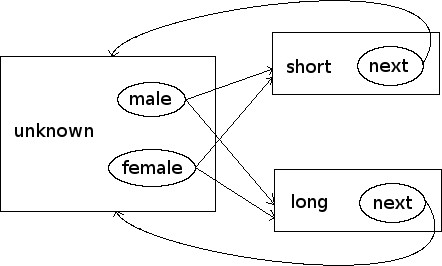
\includegraphics[width=6cm]{./ex1.jpg}
\end{figure}
\end{center}

The behaviour of the EvtStatMac is defined by the following probabilities:\\
$$P(evt:male|from:unknown)=0.5$$
$$P(evt:female|from:unknown)=0.5$$
$$P(evt:next|from:short)=1.0$$
$$P(evt:next|from:long)=1.0$$
$$P(to:short|from:unknown,evt:male)=0.9$$
$$P(to:long|from:unknown,evt:male)=0.1$$
$$P(to:short|from:unknown,evt:female)=0.5$$
$$P(to:long|from:unknown,evt:female)=0.5$$
$$P(to:unknown|from:short,evt:next)=1.0$$
$$P(to:unknown|from:long,evt:next)=1.0$$

The solution of the problem is given by: $$P(evt:male|from:unknown,to:long)$$.\\

\subsection{Code}

\begin{scriptsize}
\begin{ttfamily}
\begin{lstlisting}
#include <stdlib.h>
#include <stdio.h>
#include <math.h>
#include <time.h>
#include "evtstatmac.h"

#define rnd() (double)(rand())/(float)(RAND_MAX)
 
typedef enum {
  stat_unknownHair, stat_short, stat_long
} statusHair;
typedef enum {
  evt_male, evt_female, evt_next
} evtHair;
char *strStatHair[3] = {(char*)"unknown", 
    (char*)"ShortHair", (char*)"LongHair"};
char *strEvtHair[3] = {(char*)"Male", 
    (char*)"Female", (char*)"next"};

int main(int argc, char **argv) {
  srandom(time(NULL));
  // Create the ESM
  int nbStatus = 3;
  int nbEvent = 3;
  EvtStatMac *theESM = ESMCreate(stat_unknownHair, nbStatus, nbEvent);
  // Set the probabilities
  ESMResetNull(theESM);
  ESMSetPEvtGivFrom(theESM, stat_unknownHair, evt_male, 0.5);
  ESMSetPEvtGivFrom(theESM, stat_unknownHair, evt_female, 0.5);
  ESMSetPToGivFromEvt(theESM, stat_unknownHair, evt_male, 
    stat_short, 0.9);
  ESMSetPToGivFromEvt(theESM, stat_unknownHair, evt_male, 
    stat_long, 0.1);
  ESMSetPToGivFromEvt(theESM, stat_unknownHair, evt_female, 
    stat_short, 0.5);
  ESMSetPToGivFromEvt(theESM, stat_unknownHair, evt_female, 
    stat_long, 0.5);
  // The following probabilities are necessary to calculate P(status)
  // They represent the act of taking the next measurement in the 
  // population
  ESMSetPEvtGivFrom(theESM, stat_short, evt_next, 1.0);
  ESMSetPEvtGivFrom(theESM, stat_long, evt_next, 1.0);
  ESMSetPToGivFromEvt(theESM, stat_short, evt_next, 
    stat_unknownHair, 1.0);
  ESMSetPToGivFromEvt(theESM, stat_long, evt_next, 
    stat_unknownHair, 1.0);
  // Print the ESM
  printf("theESM:\n");
  ESMPrint(theESM, stdout, strStatHair, strEvtHair);
  // Get the probability male given long hair
  float prob = ESMGetPEvtGivFromTo(theESM, stat_unknownHair,
    evt_male, stat_long);
  printf("Probability of Male given Long hair (0.1667): %.4f\n", prob);
  // Free memory
  ESMFree(&theESM);

  return 0;
}
\end{lstlisting}
\end{ttfamily}
\end{scriptsize}

\subsection{Makefile}

\begin{scriptsize}
\begin{ttfamily}
\begin{lstlisting}
OPTIONS_DEBUG=-ggdb -g3 -Wall
OPTIONS_RELEASE=-O3 
OPTIONS=$(OPTIONS_DEBUG)

all : haircut

clean:
	rm *.o haircut
	
haircut : haircut.o evtstatmac.o Makefile
	gcc $(OPTIONS) evtstatmac.o haircut.o -o haircut -lm

haircut.o : evtstatmac.h haircut.c Makefile
	gcc $(OPTIONS) -c haircut.c

evtstatmac.o : evtstatmac.c evtstatmac.h Makefile
	gcc $(OPTIONS) -c evtstatmac.c
\end{lstlisting}
\end{ttfamily}
\end{scriptsize}

\subsection{Output}

\begin{scriptsize}
\begin{ttfamily}
\begin{lstlisting}
theESM:
current status: 'unknown'
from status 'unknown'
  by event 'Male' (0.500000):
    -> status 'ShortHair' (0.900000)
    -> status 'LongHair' (0.100000)
  by event 'Female' (0.500000):
    -> status 'ShortHair' (0.500000)
    -> status 'LongHair' (0.500000)
from status 'ShortHair'
  by event 'next' (1.000000):
    -> status 'unknown' (1.000000)
from status 'LongHair'
  by event 'next' (1.000000):
    -> status 'unknown' (1.000000)
Probability of Male given Long hair (0.1667): 0.1667
\end{lstlisting}
\end{ttfamily}
\end{scriptsize}

\section{Example 2: Disease}

\subsection{Problem definition}

The problem is as follow: a disease D affects 0.1\% of the population; a medical test for this disease identifies correctly 99\% of sick individual as having the disease and identifies incorrectly 1\% of fine individual as having the disease. We want to know the probability is to have the disease after being test positive once, and after being test positive twice.\\

This problem can be solved with a EvtStatMac as follow. We define 3 status: 'unknown', 'positive', 'negative', and 3 events: 'sick', 'fine', 'next'. It represents the following process: we test an 'unknown' person in the population, it happens to be either a 'fine', or a 'sick' person with a 'positive' or 'negative' result to the test, and we move to the 'next' 'unknown' person.\\

\begin{center}
\begin{figure}[H]
\centering
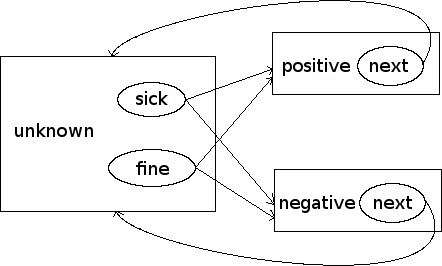
\includegraphics[width=6cm]{./ex2.jpg}
\end{figure}
\end{center}

The behaviour of the EvtStatMac is defined by the following probabilities:\\
$$P(evt:fine|from:unknown)=0.999$$
$$P(evt:sick|from:unknown)=0.001$$
$$P(evt:next|from:positive)=1.0$$
$$P(evt:next|from:negative)=1.0$$
$$P(to:positive|from:unknown,evt:fine)=0.01$$
$$P(to:negative|from:unknown,evt:fine)=0.99$$
$$P(to:positive|from:unknown,evt:sick)=0.99$$
$$P(to:negative|from:unknown,evt:sick)=0.01$$
$$P(to:unknown|from:short,evt:next)=1.0$$
$$P(to:unknown|from:long,evt:next)=1.0$$

The solution of the problem is given by: $$P(evt:sick|from:unknown,to:positive)$$ after the first positive test, then the probability $P(evt:sick|from:unknown)$ is updated with the previous result and the same probability is calculated again for the solution of the problem after the second positive test.\\

\subsection{Code}

\begin{scriptsize}
\begin{ttfamily}
\begin{lstlisting}
#include <stdlib.h>
#include <stdio.h>
#include <math.h>
#include <time.h>
#include "evtstatmac.h"

#define rnd() (double)(rand())/(float)(RAND_MAX)
 
typedef enum {
  stat_unknownDisease, stat_positive, stat_negative
} statusDisease;
typedef enum {
  evt_sick, evt_fine, evt_next
} evtDisease;
char *strStatDisease[3] = {(char*)"unknown", 
    (char*)"Positive", (char*)"Negative"};
char *strEvtDisease[3] = {(char*)"SickIndividual", 
    (char*)"FineIndividual", (char*)"next"};

int main(int argc, char **argv) {
  srandom(time(NULL));
  
  int nbState = 3;
  int nbEvent = 3;
  EvtStatMac *theESM = 
    ESMCreate(stat_unknownDisease, nbState, nbEvent);
  ESMResetNull(theESM);
  // Set the probabilities
  ESMSetPEvtGivFrom(theESM, stat_unknownDisease, 
    evt_fine, 0.999);
  ESMSetPEvtGivFrom(theESM, stat_unknownDisease, 
    evt_sick, 0.001);
  ESMSetPToGivFromEvt(theESM, stat_unknownDisease,
    evt_fine, stat_positive, 0.01);
  ESMSetPToGivFromEvt(theESM, stat_unknownDisease,
    evt_fine, stat_negative, 0.99);
  ESMSetPToGivFromEvt(theESM, stat_unknownDisease, 
    evt_sick, stat_positive, 0.99);
  ESMSetPToGivFromEvt(theESM, stat_unknownDisease, 
    evt_sick, stat_negative, 0.01);
  // The following probabilities are necessary to calculate P(status)
  // They represent the act of taking the next measurement in the 
  // population
  ESMSetPEvtGivFrom(theESM, stat_positive, evt_next, 1.0);
  ESMSetPEvtGivFrom(theESM, stat_negative, evt_next, 1.0);
  ESMSetPToGivFromEvt(theESM, stat_positive, evt_next, 
    stat_unknownDisease, 1.0);
  ESMSetPToGivFromEvt(theESM, stat_negative, evt_next, 
    stat_unknownDisease, 1.0);
  // Print the ESM
  printf("theESM:\n");
  ESMPrint(theESM, stdout, strStatDisease, strEvtDisease);
  // Get the probability of being sick given a positive test
  float prob = ESMGetPEvtGivFromTo(theESM, stat_unknownDisease,
    evt_sick, stat_positive);
  printf("Prob of Sick individual given one Positive (0.0902): %.4f\n",
    prob);
  // Update the probability of being sick with the new estimate
  printf("Update prob of Sick with previous prob\n");
  ESMSetPEvtGivFrom(theESM, stat_unknownDisease, 
    evt_fine, 1.0 - prob);
  ESMSetPEvtGivFrom(theESM, stat_unknownDisease, 
    evt_sick, prob);
  // Print the updated ESM
  printf("theESM updated:\n");
  ESMPrint(theESM, stdout, strStatDisease, strEvtDisease);
  // Get the probability of being sick given a 2nd positive test
  prob = ESMGetPEvtGivFromTo(theESM, stat_unknownDisease,
    evt_sick, stat_positive);
  printf("Prob of Sick individual given two Positive (0.9075): %.4f\n",
    prob);
  // Free memory
  ESMFree(&theESM);

  return 0;
}
\end{lstlisting}
\end{ttfamily}
\end{scriptsize}

\subsection{Makefile}

\begin{scriptsize}
\begin{ttfamily}
\begin{lstlisting}
OPTIONS_DEBUG=-ggdb -g3 -Wall
OPTIONS_RELEASE=-O3 
OPTIONS=$(OPTIONS_DEBUG)

all : disease

clean:
	rm *.o disease
	
disease : disease.o evtstatmac.o Makefile
	gcc $(OPTIONS) evtstatmac.o disease.o -o disease -lm

disease.o : evtstatmac.h disease.c Makefile
	gcc $(OPTIONS) -c disease.c

evtstatmac.o : evtstatmac.c evtstatmac.h Makefile
	gcc $(OPTIONS) -c evtstatmac.c
\end{lstlisting}
\end{ttfamily}
\end{scriptsize}

\subsection{Output}

\begin{scriptsize}
\begin{ttfamily}
\begin{lstlisting}
theESM:
current status: 'unknown'
from status 'unknown'
  by event 'SickIndividual' (0.001000):
    -> status 'Positive' (0.990000)
    -> status 'Negative' (0.010000)
  by event 'FineIndividual' (0.999000):
    -> status 'Positive' (0.010000)
    -> status 'Negative' (0.990000)
from status 'Positive'
  by event 'next' (1.000000):
    -> status 'unknown' (1.000000)
from status 'Negative'
  by event 'next' (1.000000):
    -> status 'unknown' (1.000000)
Prob of Sick individual given one Positive (0.0902): 0.0902
Update prob of Sick with previous prob
theESM updated:
current status: 'unknown'
from status 'unknown'
  by event 'SickIndividual' (0.090164):
    -> status 'Positive' (0.990000)
    -> status 'Negative' (0.010000)
  by event 'FineIndividual' (0.909836):
    -> status 'Positive' (0.010000)
    -> status 'Negative' (0.990000)
from status 'Positive'
  by event 'next' (1.000000):
    -> status 'unknown' (1.000000)
from status 'Negative'
  by event 'next' (1.000000):
    -> status 'unknown' (1.000000)
Prob of Sick individual given two Positive (0.9075): 0.9075
\end{lstlisting}
\end{ttfamily}
\end{scriptsize}

\section{Example 3: Flu epidemic}

\subsection{Problem definition}

The problem is as follow: you are in charge of some kind of medical institution treating patients of the flu and you must manage resources in prevision of the next epidemic. The epidemic are classified into 12 categories depending on the number of person having the flu in a week. You have records of the category of epidemic of the last 12 years for each week of these year. You need to run simulation of epidemics for training, and forecast the probabilities of categories of current epidemic 3 weeks in advance to get prepared to trigger a special epidemic plan in certain condition.\\

This problem can be solved with a EvtStatMac as follow. We define as many status as there are categories, and as many events as there are weeks. It represents the following process: The EvtStatMac current status is the category of current epidemic from which the event corresponding to 'moving to next week' changes the status to the category of the epidemic at the following week.\\

The behaviour of the EvtStatMac is learnt from real data for flu epidemic in France from 2003 to 2015 ("Data Source: Google Flu Trends (http://www.google.org/flutrends)"). Category $c$ is defined as $c*100\le n<(c+1)*100$ where $n$ is the number of people having the flu during a given week.\\

Simulation can be run by using the {\ttfamily ESMStep()} function, and forecast for outbreak can be calculated with {\ttfamily ESMGetPToGivFrom()}.\\

\subsection{Code}

\begin{scriptsize}
\begin{ttfamily}
\begin{lstlisting}
#include <stdlib.h>
#include <stdio.h>
#include <math.h>
#include <time.h>
#include "evtstatmac.h"
#include "tga.h"

#define rnd() (double)(rand())/(float)(RAND_MAX)
 
typedef enum {
  stat_0, stat_1, stat_2, stat_3, stat_4, stat_5, 
  stat_6, stat_7, stat_8, stat_9, stat_10, stat_11
} statusEpidemic;
typedef enum {
  evt_toWeek1, evt_toWeek2, evt_toWeek3, evt_toWeek4, evt_toWeek5,
  evt_toWeek6, evt_toWeek7, evt_toWeek8, evt_toWeek9, evt_toWeek10,
  evt_toWeek11, evt_toWeek12, evt_toWeek13, evt_toWeek14, evt_toWeek15,
  evt_toWeek16, evt_toWeek17, evt_toWeek18, evt_toWeek19, evt_toWeek20,
  evt_toWeek21, evt_toWeek22, evt_toWeek23, evt_toWeek24, evt_toWeek25,
  evt_toWeek26, evt_toWeek27, evt_toWeek28, evt_toWeek29, evt_toWeek30,
  evt_toWeek31, evt_toWeek32, evt_toWeek33, evt_toWeek34, evt_toWeek35,
  evt_toWeek36, evt_toWeek37, evt_toWeek38, evt_toWeek39, evt_toWeek40,
  evt_toWeek41, evt_toWeek42, evt_toWeek43, evt_toWeek44, evt_toWeek45,
  evt_toWeek46, evt_toWeek47, evt_toWeek48, evt_toWeek49, evt_toWeek50,
  evt_toWeek51, evt_toWeek52, evt_toWeek53
} evtEpidemic;
char *strStatEpidemic[12] = {
  (char*)"Cat 0", (char*)"Cat 1", (char*)"Cat 2", (char*)"Cat 3", 
  (char*)"Cat 4", (char*)"Cat 5", (char*)"Cat 6", 
  (char*)"Cat 7", (char*)"Cat 8", (char*)"Cat 9", 
  (char*)"Cat 10", (char*)"Cat 11"
};
char *strEvtEpidemic[53] = {
  (char*)"toWeek1", (char*)"toWeek2", (char*)"toWeek3", 
  (char*)"toWeek4", (char*)"toWeek5", (char*)"toWeek6", 
  (char*)"toWeek7", (char*)"toWeek8", (char*)"toWeek9", 
  (char*)"toWeek10", 
  (char*)"toWeek11", (char*)"toWeek12", (char*)"toWeek13", 
  (char*)"toWeek14", (char*)"toWeek15", (char*)"toWeek16",
  (char*)"toWeek17", (char*)"toWeek18", (char*)"toWeek19", 
  (char*)"toWeek20", 
  (char*)"toWeek21", (char*)"toWeek22", (char*)"toWeek23", 
  (char*)"toWeek24", (char*)"toWeek25", (char*)"toWeek26",
  (char*)"toWeek27", (char*)"toWeek28", (char*)"toWeek29", 
  (char*)"toWeek30", 
  (char*)"toWeek31", (char*)"toWeek32", (char*)"toWeek33", 
  (char*)"toWeek34", (char*)"toWeek35", (char*)"toWeek36", 
  (char*)"toWeek37", (char*)"toWeek38", (char*)"toWeek39", 
  (char*)"toWeek40", 
  (char*)"toWeek41", (char*)"toWeek42", (char*)"toWeek43", 
  (char*)"toWeek44", (char*)"toWeek45", (char*)"toWeek46", 
  (char*)"toWeek47", (char*)"toWeek48", (char*)"toWeek49", 
  (char*)"toWeek50", 
  (char*)"toWeek51", (char*)"toWeek52", (char*)"toWeek53"
};
int nbSampleEpidemic = 619;
int dataEpidemic[1857] = {
  4,41,4,4,42,4,4,43,6,6,44,6,6,45,5,5,46,7,7,47,8,8,48,9,9,49,10,10,
  50,9,9,51,8,8,52,8,8,1,7,7,2,6,6,3,5,5,4,4,4,5,4,4,6,5,5,7,4,4,8,4,
  4,9,4,4,10,4,4,11,4,4,12,3,3,13,3,3,14,3,3,15,3,3,16,3,3,17,2,2,18,
  3,3,19,3,3,20,3,3,21,2,2,22,2,2,23,3,3,24,2,2,25,2,2,26,2,2,27,2,2,
  28,2,2,29,2,2,30,2,2,31,2,2,32,2,2,33,3,3,34,2,2,35,3,3,36,2,2,37,3,
  3,38,3,3,39,5,5,40,5,5,41,5,5,42,5,5,43,5,5,44,5,5,45,5,5,46,5,5,47,
  5,5,48,5,5,49,6,6,50,6,6,51,6,6,52,7,7,1,7,7,2,7,7,3,7,7,4,7,7,5,8,
  8,6,9,9,7,10,10,8,9,9,9,8,8,10,7,7,11,7,7,12,6,6,13,6,6,14,5,5,15,
  5,5,16,4,4,17,4,4,18,4,4,19,3,3,20,3,3,21,3,3,22,3,3,23,3,3,24,3,3,
  25,3,3,26,3,3,27,2,2,28,2,2,29,2,2,30,3,3,31,3,3,32,3,3,33,3,3,34,3,
  3,35,3,3,36,3,3,37,3,3,38,4,4,39,5,5,40,5,5,41,6,6,42,6,6,43,6,6,44,
  5,5,45,5,5,46,6,6,47,6,6,48,6,6,49,6,6,50,6,6,51,6,6,52,6,6,53,6,6,
  1,6,6,2,6,6,3,6,6,4,7,7,5,7,7,6,8,8,7,7,7,8,7,7,9,6,6,10,6,6,11,6,6,
  12,5,5,13,5,5,14,5,5,15,4,4,16,4,4,17,4,4,18,3,3,19,3,3,20,3,3,21,3,
  3,22,3,3,23,3,3,24,2,2,25,2,2,26,2,2,27,2,2,28,2,2,29,2,2,30,2,2,31,
  2,2,32,2,2,33,3,3,34,3,3,35,3,3,36,3,3,37,3,3,38,4,4,39,4,4,40,4,4,
  41,5,5,42,5,5,43,5,5,44,5,5,45,5,5,46,5,5,47,5,5,48,5,5,49,6,6,50,6,
  6,51,6,6,52,7,7,1,7,7,2,7,7,3,7,7,4,7,7,5,8,8,6,9,9,7,8,8,8,7,7,9,6,
  6,10,5,5,11,4,4,12,4,4,13,4,4,14,4,4,15,4,4,16,3,3,17,2,2,18,2,2,19,
  2,2,20,2,2,21,2,2,22,3,3,23,3,3,24,2,2,25,2,2,26,2,2,27,2,2,28,2,2,
  29,2,2,30,2,2,31,2,2,32,2,2,33,2,2,34,2,2,35,2,2,36,3,3,37,3,3,38,4,
  4,39,5,5,40,5,5,41,5,5,42,5,5,43,6,6,44,5,5,45,6,6,46,6,6,47,6,6,48,
  6,6,49,6,6,50,6,6,51,7,7,52,7,7,1,8,8,2,8,8,3,8,8,4,8,8,5,8,8,6,8,8,
  7,8,8,8,7,7,9,6,6,10,6,6,11,5,5,12,5,5,13,5,5,14,5,5,15,4,4,16,4,4,
  17,4,4,18,3,3,19,2,2,20,2,2,21,2,2,22,2,2,23,3,3,24,3,3,25,3,3,26,2,
  2,27,2,2,28,2,2,29,2,2,30,2,2,31,2,2,32,2,2,33,2,2,34,2,2,35,2,2,36,
  2,2,37,3,3,38,4,4,39,5,5,40,5,5,41,5,5,42,5,5,43,5,5,44,5,5,45,5,5,
  46,5,5,47,5,5,48,5,5,49,6,6,50,6,6,51,7,7,52,8,8,1,9,9,2,9,9,3,9,9,
  4,9,9,5,8,8,6,7,7,7,6,6,8,5,5,9,5,5,10,4,4,11,4,4,12,4,4,13,4,4,14,
  4,4,15,3,3,16,3,3,17,3,3,18,3,3,19,3,3,20,3,3,21,3,3,22,2,2,23,2,2,
  24,2,2,25,3,3,26,2,2,27,2,2,28,2,2,29,3,3,30,4,4,31,4,4,32,4,4,33,3,
  3,34,4,4,35,5,5,36,5,5,37,6,6,38,7,7,39,6,6,40,7,7,41,6,6,42,6,6,43,
  6,6,44,7,7,45,7,7,46,7,7,47,8,8,48,9,9,49,9,9,50,9,9,51,8,8,52,7,7,1,
  7,7,2,7,7,3,6,6,4,5,5,5,5,5,6,5,5,7,5,5,8,4,4,9,4,4,10,3,3,11,3,3,
  12,3,3,13,3,3,14,3,3,15,3,3,16,2,2,17,2,2,18,2,2,19,2,2,20,2,2,21,
  2,2,22,2,2,23,2,2,24,1,1,25,1,1,26,1,1,27,1,1,28,1,1,29,1,1,30,1,1,
  31,1,1,32,1,1,33,1,1,34,2,2,35,2,2,36,2,2,37,2,2,38,4,4,39,4,4,40,5,
  5,41,4,4,42,4,4,43,4,4,44,4,4,45,4,4,46,3,3,47,4,4,48,4,4,49,5,5,50,
  5,5,51,6,6,52,7,7,1,8,8,2,8,8,3,8,8,4,8,8,5,8,8,6,8,8,7,7,7,8,7,7,9,
  5,5,10,5,5,11,4,4,12,3,3,13,3,3,14,3,3,15,3,3,16,2,2,17,2,2,18,1,1,
  19,1,1,20,1,1,21,1,1,22,1,1,23,1,1,24,1,1,25,1,1,26,1,1,27,1,1,28,1,
  1,29,1,1,30,1,1,31,1,1,32,1,1,33,1,1,34,1,1,35,1,1,36,1,1,37,1,1,38,
  2,2,39,3,3,40,4,4,41,4,4,42,4,4,43,4,4,44,4,4,45,4,4,46,4,4,47,5,5,
  48,5,5,49,5,5,50,5,5,51,5,5,52,5,5,53,6,6,1,6,6,2,5,5,3,6,6,4,6,6,5,
  6,6,6,7,7,7,8,8,8,8,8,9,8,8,10,7,7,11,6,6,12,5,5,13,4,4,14,4,4,15,4,
  4,16,3,3,17,3,3,18,2,2,19,2,2,20,2,2,21,2,2,22,2,2,23,1,1,24,1,1,25,
  2,2,26,1,1,27,1,1,28,2,2,29,2,2,30,1,1,31,1,1,32,1,1,33,1,1,34,1,1,
  35,1,1,36,2,2,37,2,2,38,4,4,39,5,5,40,5,5,41,5,5,42,5,5,43,5,5,44,5,
  5,45,5,5,46,5,5,47,5,5,48,5,5,49,6,6,50,6,6,51,7,7,52,8,8,1,8,8,2,8,
  8,3,8,8,4,9,9,5,10,10,6,10,10,7,10,10,8,9,9,9,8,8,10,7,7,11,6,6,12,5,
  5,13,5,5,14,5,5,15,4,4,16,3,3,17,3,3,18,3,3,19,3,3,20,2,2,21,3,3,22,
  3,3,23,2,2,24,2,2,25,2,2,26,2,2,27,1,1,28,1,1,29,1,1,30,0,0,31,0,0,
  32,1,1,33,1,1,34,1,1,35,1,1,36,1,1,37,2,2,38,4,4,39,5,5,40,4,4,41,4,
  4,42,4,4,43,4,4,44,4,4,45,4,4,46,4,4,47,5,5,48,5,5,49,5,5,50,6,6,51,
  6,6,52,6,6,1,6,6,2,6,6,3,6,6,4,6,6,5,7,7,6,8,8,7,8,8,8,8,8,9,7,7,10,
  6,6,11,5,5,12,5,5,13,4,4,14,4,4,15,4,4,16,3,3,17,3,3,18,3,3,19,2,2,
  20,2,2,21,2,2,22,2,2,23,2,2,24,1,1,25,1,1,26,1,1,27,1,1,28,1,1,29,1,
  1,30,1,1,31,1,1,32,1,1,33,1,1,34,2,2,35,1,1,36,1,1,37,2,2,38,3,3,39,
  4,4,40,4,4,41,4,4,42,4,4,43,4,4,44,4,4,45,4,4,46,4,4,47,5,5,48,5,5,
  49,5,5,50,6,6,51,6,6,52,7,7,1,7,7,2,7,7,3,7,7,4,8,8,5,10,10,6,11,11,
  7,11,11,8,11,11,9,9,9,10,7,7,11,6,6,12,5,5,13,5,5,14,4,4,15,4,4,16,
  3,3,17,3,3,18,2,2,19,2,2,20,2,2,21,2,2,22,2,2,23,2,2,24,2,2,25,2,2,
  26,1,1,27,0,0,28,0,0,29,0,0,30,0,0,31,1,1,32,0,0,33,1
};

int main(int argc, char **argv) {
  srandom(time(NULL));
  
  // Create the ESM
  int nbState = 12;
  int nbEvent = 53;
  EvtStatMac *epidemicESM = ESMCreate(stat_0, nbState, nbEvent);
  // Learn from samples
  printf("Learning from epidemic data\n");
  ESMResetNull(epidemicESM);
  for (int iSample = 0; iSample < nbSampleEpidemic; ++iSample) {
    esmStat from = dataEpidemic[3 * iSample];
    esmEvt event = dataEpidemic[3 * iSample + 1] - 1;
    esmStat to = dataEpidemic[3 * iSample + 2];
    ESMLearn(epidemicESM, from, event, to);
  }
  // Create artificial data sample and save as a graph
  // with samples as background
  printf("Artificial data series (week/category):\n");
  TGA *graph = NULL;
  short coeff[2] = {4, 10};
  short dim[2];
  dim[0] = coeff[0] * nbEvent;
  dim[1] = coeff[1] * nbState;
  TGAPixel pix;
  pix._rgba[0] = pix._rgba[1] = pix._rgba[2] = 255;
  pix._rgba[3] = 255;
  graph = TGACreate(dim, &pix);
  TGAPencil *pen = TGAGetBlackPencil();
  if (graph == NULL) {
    fprintf(stderr, "Error while creating the graph\n");
    ESMFree(&epidemicESM);
    return 1;
  }
  float fromPx[2];
  float toPx[2];
  pix._rgba[0] = pix._rgba[1] = 155;
  TGAPencilSetColor(pen, &pix);
  for (int iSample = 0; iSample < nbSampleEpidemic - 1; ++iSample) {
    esmStat from = dataEpidemic[3 * iSample];
    esmEvt event = dataEpidemic[3 * iSample + 1];
    esmStat to = dataEpidemic[3 * iSample + 2];
    if (event > 1) {
      fromPx[0] = (event - 1) * coeff[0];
      fromPx[1] = from * coeff[1];
      toPx[0] = event * coeff[0];
      toPx[1] = to * coeff[1];
      TGADrawLine(graph, fromPx, toPx, pen);
    }
  }
  epidemicESM->_curState = stat_7;
  pix._rgba[0] = pix._rgba[1] = pix._rgba[2] = 0;
  TGAPencilSetColor(pen, &pix);
  for (int iWeek = 1; iWeek < 52; ++iWeek) {
    esmStat curStat = ESMGetStat(epidemicESM);
    if (curStat == ESM_STATNULL) {
      printf("Unexpected situation");
      iWeek = 53;
    } else {
      ESMStepByEvt(epidemicESM, iWeek);
      esmStat nextStat = ESMGetStat(epidemicESM);
      fromPx[0] = (iWeek - 1) * coeff[0];
      fromPx[1] = curStat * coeff[1];
      toPx[0] = iWeek * coeff[0];
      toPx[1] = nextStat * coeff[1];
      TGADrawLine(graph, fromPx, toPx, pen);
      printf("%d/%s, ", iWeek, strStatEpidemic[curStat]);
    }
  }
  printf("\n");
  TGAGaussBlur(graph, 0.5, 2.0);
  TGASave(graph, (char*)"./graph.tga");
  TGAFree(&graph);
  // Forecast probability from week 48, 3 weeks ahead
  printf("Example of helping management of epidemic special plan.\n");
  printf("Check if (prob of cat. 8+) > 25%% in 3 weeks.\n");
  esmEvt fromWeek = 48;
  esmStat fromStat = stat_5;
  int thresholdCat = 8;
  float threshold = 0.25;
  int nbWeek = 3;
  bool flagAlert = false;
  // Create a clone and delete all the transitions out of the period 
  // to create a submodel of the epidemic during the relevant weeks
  EvtStatMac *clone = ESMClone(epidemicESM);
  for (int from = 0; from < clone->_nbStatus; ++from) {
    for (int event = 0; event < clone->_nbEvent; ++event) {
      for (int to = 0; to < clone->_nbStatus; ++to) {
        if (event < fromWeek || event > fromWeek + nbWeek) {
          ESMSetPToGivFromEvt(clone, from, event, to, 0.0);
        }
      }
    }
  }
  // Renormalize the ESM
  ESMNormalize(clone);
  // Get the probabilities for each category
  printf("At week %d with a current category of %s, %d weeks forecast:\n", 
    fromWeek, strStatEpidemic[fromStat], nbWeek);
  flagAlert = false;
  for (int to = 0; to < clone->_nbStatus; ++to) {
    float prob = 
      ESMGetPToGivFrom(clone, fromStat, to, nbWeek);
    if (prob > ESM_EPSILON) {
      printf("  to %s: %.3f\n", strStatEpidemic[to], prob);
      if (to >= thresholdCat && prob > threshold)
        flagAlert = true;
    }
  }
  if (flagAlert == false)
    printf("  -> No need to trigger the epidemic plan.\n");
  else
    printf("  -> Need to trigger the epidemic plan.\n");
  // One week later, if situation hasn't changed
  fromWeek += 1;
  // Create another clone and delete all the transitions out of the period 
  // to create a submodel of the epidemic during the relevant weeks
  ESMFree(&clone);
  clone = ESMClone(epidemicESM);
  for (int from = 0; from < clone->_nbStatus; ++from) {
    for (int event = 0; event < clone->_nbEvent; ++event) {
      for (int to = 0; to < clone->_nbStatus; ++to) {
        if (event < fromWeek || event > fromWeek + nbWeek) {
          ESMSetPToGivFromEvt(clone, from, event, to, 0.0);
        }
      }
    }
  }
  // Renormalize the ESM
  ESMNormalize(clone);
  // Get the probabilities for each category
  printf("Next week (%d) with category unchanged, %d weeks forecast:\n", 
    fromWeek, nbWeek);
  flagAlert = false;
  for (int to = 0; to < clone->_nbStatus; ++to) {
    float prob = 
      ESMGetPToGivFrom(clone, fromStat, to, nbWeek);
    if (prob > ESM_EPSILON) {
      printf("  to %s: %.3f\n", strStatEpidemic[to], prob);
      if (to >= thresholdCat && prob > threshold)
        flagAlert = true;
    }
  }
  if (flagAlert == false)
    printf("  -> No need to trigger the epidemic plan.\n");
  else
    printf("  -> Need to trigger the epidemic plan.\n");
  // One week later, if situation has deteriorated
  fromStat += 1;
  // Get the probabilities for each category
  printf("If the category had been %s:\n", strStatEpidemic[fromStat]);
  flagAlert = false;
  for (int to = 0; to < clone->_nbStatus; ++to) {
    float prob = 
      ESMGetPToGivFrom(clone, fromStat, to, nbWeek);
    if (prob > ESM_EPSILON) {
      printf("  to %s: %.3f\n", strStatEpidemic[to], prob);
      if (to >= thresholdCat && prob > threshold)
        flagAlert = true;
    }
  }
  if (flagAlert == false)
    printf("  -> No need to trigger the epidemic plan.\n");
  else
    printf("  -> Need to trigger the epidemic plan.\n");
  // Free memory
  ESMFree(&epidemicESM);
  ESMFree(&clone);

  return 0;
}
\end{lstlisting}
\end{ttfamily}
\end{scriptsize}

\subsection{Makefile}

\begin{scriptsize}
\begin{ttfamily}
\begin{lstlisting}
OPTIONS_DEBUG=-ggdb -g3 -Wall
OPTIONS_RELEASE=-O3 
OPTIONS=$(OPTIONS_DEBUG)
INCPATH=./Include
LIBPATH=./Lib

all : epidemic

clean:
	rm *.o epidemic
	
epidemic : epidemic.o evtstatmac.o Makefile
	gcc $(OPTIONS) $(LIBPATH)/tgapaint.o evtstatmac.o epidemic.o -o epidemic -lm

epidemic.o : evtstatmac.h epidemic.c Makefile $(INCPATH)/tgapaint.h
	gcc $(OPTIONS) -I$(INCPATH) -c epidemic.c

evtstatmac.o : evtstatmac.c evtstatmac.h Makefile
	gcc $(OPTIONS) -c evtstatmac.c
\end{lstlisting}
\end{ttfamily}
\end{scriptsize}

\subsection{Output}

\begin{scriptsize}
\begin{ttfamily}
\begin{lstlisting}
Learning from epidemic data
Artificial data series (week/category):
1/Cat 7, 2/Cat 7, 3/Cat 7, 4/Cat 7, 5/Cat 8, 6/Cat 9, 7/Cat 8, 8/Cat 8, 
9/Cat 8, 10/Cat 7, 11/Cat 7, 12/Cat 6, 13/Cat 6, 14/Cat 5, 15/Cat 5, 
16/Cat 4, 17/Cat 4, 18/Cat 3, 19/Cat 3, 20/Cat 2, 21/Cat 3, 22/Cat 2, 
23/Cat 2, 24/Cat 2, 25/Cat 2, 26/Cat 2, 27/Cat 1, 28/Cat 1, 29/Cat 1, 
30/Cat 1, 31/Cat 1, 32/Cat 1, 33/Cat 1, 34/Cat 2, 35/Cat 3, 36/Cat 3, 
37/Cat 3, 38/Cat 3, 39/Cat 5, 40/Cat 5, 41/Cat 5, 42/Cat 5, 43/Cat 5, 
44/Cat 5, 45/Cat 5, 46/Cat 5, 47/Cat 5, 48/Cat 5, 49/Cat 6, 50/Cat 6, 
51/Cat 6, 
Example of helping management of epidemic special plan.
Check if (prob of cat. 8+) > 25% in 3 weeks.
At week 48 with a current category of Cat 5, 3 weeks forecast:
  to Cat 5: 0.110
  to Cat 6: 0.527
  to Cat 7: 0.278
  to Cat 8: 0.084
  -> No need to trigger the epidemic plan.
Next week (49) with category unchanged, 3 weeks forecast:
  to Cat 5: 0.131
  to Cat 6: 0.508
  to Cat 7: 0.278
  to Cat 8: 0.083
  -> No need to trigger the epidemic plan.
If the category had been Cat 6:
  to Cat 6: 0.290
  to Cat 7: 0.401
  to Cat 8: 0.309
  -> Need to trigger the epidemic plan.
\end{lstlisting}
\end{ttfamily}
\end{scriptsize}

Graphics of 4 simulations of flu epidemic (real data in blue, simulation in black, weeks in abciss, category in ordinate):\\
\begin{center}
\begin{figure}[H]
\centering
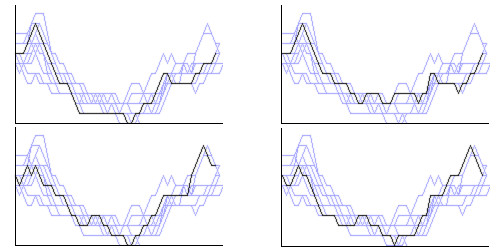
\includegraphics[width=10cm]{./flu.jpg}
\end{figure}
\end{center}

\newpage
\section{Annex 1}
\label{proofA}
Proof of $P(e,s'|s)=P(s'|s,e)P(e|s)$\\
We have:\\
$$
P(s,e,s')=P(s)P(e|s)P(s'|s,e)\\
$$
and\\
$$
P(e,s'|s)=\frac{P(s,e,s')}{P(s)}
$$
then\\
$$
\begin{array}{ll}
P(e,s'|s)&=\frac{P(s'|s,e)P(e|s)P(s)}{P(s)}\\
&=P(s'|s,e)P(e|s)\\
\end{array}
$$

\end{document}

\section{Example 4: Cashier}

\subsection{Code}

\begin{scriptsize}
\begin{ttfamily}
\begin{lstlisting}

\end{lstlisting}
\end{ttfamily}
\end{scriptsize}

\subsection{Makefile}

\begin{scriptsize}
\begin{ttfamily}
\begin{lstlisting}

\end{lstlisting}
\end{ttfamily}
\end{scriptsize}

\subsection{Output}

\begin{scriptsize}
\begin{ttfamily}
\begin{lstlisting}

\end{lstlisting}
\end{ttfamily}
\end{scriptsize}

